\documentclass[A4wide,12pt]{report}

\DeclareUnicodeCharacter{202F}{\,}

%\usepackage{arabtex}  % removed: conflicts with [utf8]{inputenc}
%\usepackage{utf8}     % removed: conflicts with [utf8]{inputenc}
%\setcode{utf8}        % removed: conflicts with [utf8]{inputenc}
\usepackage{tikz}
\usepackage[font={small,it}]{caption}
\usepackage[french]{minitoc}
\usepackage[utf8]{inputenc}
\usepackage[french]{babel}
\usepackage[T1]{fontenc}
\usepackage{a4wide,indentfirst}
\usepackage{pdflscape}
\usepackage{graphicx}
\graphicspath{{Figures/}{Figures/Chapitre1/}{Figures/Chapitre2/}{Figures/Chapitre3/}{Figures/Chapitre4/}{Figures/Chapitre5/}}
\usepackage{fancyhdr}
\setlength{\headheight}{28pt}
\usepackage{enumitem}
\usepackage{lastpage}
\usepackage{setspace}
\setcounter{tocdepth}{4}
\setcounter{secnumdepth}{4}
\usepackage{longtable}
\usepackage{subfigure}
\usepackage{graphics}
\usepackage{colortbl}
\usepackage{xcolor}
\usepackage[hidelinks]{hyperref}
\usepackage{listings}
\usepackage{pdfpages}
\usepackage{float}
\usepackage{footnote}
\usepackage[bottom]{footmisc}
\usepackage[a4paper,margin=2.5cm]{geometry}
\usepackage{url}
\usepackage{multirow}
\usepackage{lipsum}
\usepackage{wrapfig}
\usepackage{cleveref}
\usepackage[export]{adjustbox}
\usepackage{color}


\linespread{1.5}
\setcounter{secnumdepth}{4}
\DeclareUnicodeCharacter{0301}{\'{e}}

% Configuration minitoc (dans le préambule, SANS \dominitoc)
\mtcsettitle{minitoc}{Plan}
\mtcsetrules{minitoc}{off}
\mtcsetfeature{minitoc}{before}{\vspace{-20pt}}

% CODE LISTING CONFIGURATION
\lstset{
    basicstyle=\small,
    breakindent=10pt,
    breaklines=true,
    captionpos=b,
    columns=fullflexible,
    commentstyle=\sffamily\slshape\color[gray]{0.5},
    frame=l,
    stringstyle=\mdseries\rmfamily,
    tabsize=2,
    xleftmargin=16pt,
    xrightmargin=20pt,
    escapeinside={*'}{'*},
    language=Python,
    breaklines=true,
}

% HYPERSETUP
\hypersetup{
    breaklinks=true,
    urlcolor=blue,
    linkcolor=blue,
    bookmarksopen=true,
    pdftitle={{Application Web de Gestion du Service Après-Vente (SAV Manager)}},
    pdfauthor={{Hend Kharrat}},
    pdfsubject={{Projet de Fin d'Études -- EDI Solutions}}
}

% COLORS
\definecolor{color_29791}{rgb}{0,0,0}
\definecolor{color_277797}{rgb}{0.988235,0.760784,0}
\definecolor{color_32005}{rgb}{0,0.262745,0.537255}
\definecolor{color_70400}{rgb}{0.156863,0.258824,0.482353}

% CUSTOM CHAPTER STYLE (black box)
\makeatletter
\newlength{\chapter@number@width}
\def\@makechapterhead#1{%
  {\normalfont
  \setlength{\parindent}{0pt}
  \vspace*{10pt}
  \settowidth{\chapter@number@width}{%
    \hbox{\color{white}\Large\bfseries
          \hspace{\dimexpr 1mm+3pt}%
          \thechapter
          \hspace{\dimexpr 1mm+3pt}%
    }}
  \hbox{%
    \vtop{%
      \hsize=\dimexpr\chapter@number@width+\tabcolsep+2\fboxrule+\tabcolsep
      \begin{tabular}[t]{@{}c}
        \scshape\strut\makebox[0pt]{\hspace{-50pt plus 1 fill minus 1 fill}\@chapapp\hspace{0pt plus 1 fill minus 1 fill}}
        \fboxsep=0pt
        \colorbox{black}{\vbox{%
           \hbox{\vbox to 1cm{}}
           \hbox{\color{white}\LARGE\bfseries
                 \hspace{\dimexpr 1mm+3pt}%
                 \thechapter
                 \hspace{\dimexpr 1mm+3pt}%
                }
           \hrule height 0.4pt depth 0pt width 0pt
           \hbox{\vbox to 6pt{}}
           \hbox{\parbox{0pt}{\Large\bfseries\vphantom{E}}}
           }}%
      \end{tabular}%
      }%
    \vtop{%
      \advance\hsize by -\dimexpr\chapter@number@width+2\fboxrule+\tabcolsep
      \hspace*{-0.5cm}\begin{tabular}[t]{c}
        \scshape\strut\vphantom{\@chapapp}
        \fboxsep=0pt
        \colorbox{white}{\vbox{%
           \hbox{\vbox to \dimexpr 1mm+3pt{}}
           \hbox{\LARGE\bfseries
                 \hspace{\dimexpr 1mm+3pt}%
                 \phantom{\thechapter}
                 \hspace{\dimexpr 1mm+3pt}%
                }
           \hrule height 0.4pt depth 0pt width \hsize
           \hbox{\vbox to 6pt{}}
           \hbox{\hspace*{20pt}\parbox{\dimexpr\textwidth-2mm-6pt-\chapter@number@width-\tabcolsep-2\fboxrule-20pt}{\Large\bfseries #1}}
           }}%
      \end{tabular}%
      }%
    }%
  \vspace{50pt}%
  }
}
\makeatother

% Réduction de l'espace vertical avant les titres de chapitres non numérotés
% (Introduction, Conclusion, Perspectives, Webographie, TOC, listes)
% Sans titlesec pour ne pas écraser le style personnalisé \@makechapterhead
\makeatletter
\def\@makeschapterhead#1{%
  \vspace*{-60pt}%
  {\parindent \z@ \raggedright
    \normalfont
    \interlinepenalty\@M
    \Huge \bfseries #1\par\nobreak
    \vskip 25\p@
  }}
\makeatother

\sloppy

\begin{document}

\pagenumbering{roman}

\rhead{\emph{}}

% ===== TITLE PAGE =====
% TODO: ajouter la page de garde finale PDF ici

\includepdf[pages=-]{page-de-garde.pdf}

\setstretch{1.5}

% ===== FRONT MATTER =====
\newpage
\section*{Remerciements}
\addcontentsline{toc}{section}{Remerciements}

\textit{[À compléter]}

\newpage
\thispagestyle{empty}
\section*{Dédicace}
\addcontentsline{toc}{section}{Dédicace}

\vspace{1cm}

\begin{center}

Je dédie ce modeste travail à ceux qui ont été ma force, mon soutien et ma source de motivation tout au long de mon parcours.

À mon cher père, \textbf{Mohamed Kharrat},

Pour tous les sacrifices consentis, ton soutien constant et la confiance que tu m'as toujours accordée. Je te témoigne mon profond respect et ma sincère gratitude.

À ma très chère mère, \textbf{Mouna},

Pour ton amour inconditionnel, ta patience et ta présence permanente à mes côtés. Merci d'avoir toujours été là pour moi, dans les moments de joie comme dans les moments difficiles. Cette réussite est aussi la tienne.

À mon fiancé, \textbf{Mahmoud Kchaou},

Pour ton soutien précieux, ta confiance en moi et l'immense motivation que tu m'as apportée. Merci de m'avoir encouragée à persévérer et à croire en mes capacités lorsque j'en avais le plus besoin.

À mes chers frères, \textbf{Hedi}, \textbf{Abdou} et \textbf{Kayen},

Pour leur affection, leurs encouragements et tous les beaux moments partagés.

À tous ceux qui ont contribué, de près ou de loin, à la réalisation de ce projet.

Avec tout mon amour, ma reconnaissance et mon respect.

\end{center}



% ===== TABLE OF CONTENTS =====
\dominitoc  % ← À placer impérativement AVANT \tableofcontents

\cleardoublepage
\begingroup
\makeatletter
\let\ps@plain\ps@empty
\makeatother
\pagestyle{empty}

\tableofcontents
\cleardoublepage

\listoffigures
\cleardoublepage

\listoftables
\cleardoublepage

\endgroup
\pagestyle{fancy}

% ===== MAIN CONTENT =====
\pagenumbering{arabic}

\cleardoublepage
\phantomsection
\addcontentsline{toc}{chapter}{Introduction Générale}
\chapter*{Introduction Générale}
\mtcaddchapter

Aujourd’hui, les entreprises évoluent dans un environnement marqué par une transformation numérique rapide, les poussant à moderniser leurs méthodes de gestion afin d’améliorer leur efficacité et la qualité de leurs services. Dans ce contexte, la centralisation des données et l’automatisation des processus deviennent des éléments essentiels pour assurer un meilleur suivi des activités et une prise de décision plus efficace.

Le service après-vente (SAV), notamment dans le domaine de la maintenance technique, repose sur la gestion des clients, des équipements, des contrats et des interventions. Cependant, ces opérations sont souvent gérées de manière traditionnelle, ce qui entraîne des difficultés de suivi, un manque de coordination entre les acteurs et un risque d’erreurs ou de perte d’information.

Ce projet de fin d’études vise à concevoir et développer une application web de gestion du service après-vente dédiée à la maintenance des climatiseurs et des systèmes de surpression. L’objectif principal est de centraliser les informations, d’optimiser la gestion des interventions et d’améliorer la traçabilité des opérations ainsi que la communication entre les différents utilisateurs du système.

Afin de mener à bien ce projet, la méthodologie Scrum a été adoptée. Elle permet un développement itératif et progressif du système à travers plusieurs sprints, tout en garantissant une meilleure adaptation aux besoins et une amélioration continue du produit.

\begin{enumerate}
    \item Le \textbf{premier chapitre} présente l'étude préalable, le contexte du projet, ainsi que
          la problématique et la solution proposée.
    \item Le \textbf{deuxième chapitre} est consacré à la capture et la spécification des besoins.
    \item Le \textbf{troisième chapitre} traite le Sprint 1 : Authentification et référentiel métier.
    \item Le \textbf{quatrième chapitre} traite le Sprint 2 : Gestion des interventions.
    \item Le \textbf{cinquième chapitre} traite le Sprint 3 : Facturation et tableau de bord.
\end{enumerate}

\newpage

\newpage
\pagestyle{fancy}
\lhead{\textsc{Chapitre 1. Étude préalable}}
\renewcommand{\headrulewidth}{0.5pt}
\renewcommand{\footrulewidth}{0.5pt}
\chapter{Étude préalable}\setlength{\headheight}{28pt}
\label{ch1}
\thispagestyle{empty}
\minitoc
\newpage

\section{Introduction}

Ce premier chapitre pose les bases du projet en présentant l'organisme d'accueil, le cadre du stage,
l'analyse de l'existant, la problématique identifiée et la solution proposée. Il constitue le fondement
sur lequel repose l'ensemble des décisions de conception et de développement.

% ─────────────────────────────────────────────────────────────────────────────
\section{Présentation de l'organisme d'accueil}

\subsection{Historique}

EDI SOLUTIONS est une entreprise spécialisée dans les services d'ingénierie informatique et les
solutions digitales. Elle a été créée pour aider les entreprises à se transformer numériquement en
développant des solutions adaptées à leurs besoins. Au fil du temps, elle a élargi ses activités pour
inclure le développement web, l'intégration de systèmes d'information et les solutions ERP.

\begin{figure}[H]
    \centering
    
\includegraphics[width=0.2\textwidth]{Figures/logo_societe.png}
    \caption{Logo d'EDI SOLUTIONS}
    \label{fig:logo_societe}
\end{figure}

\subsection{Domaine d'activité}

L'entreprise opère principalement dans le secteur des technologies de l'information et de la
communication. Ses activités incluent :

\begin{itemize}
    \item Le conseil et l'audit des systèmes d'information ;
    \item Le développement d'applications web et mobiles ;
    \item L'intégration de solutions ERP et cloud ;
    \item La mise en place de systèmes d'information sur mesure.
\end{itemize}

\subsection{Positionnement}

L'entreprise se positionne comme un fournisseur de solutions numériques innovantes, capable de répondre
aux besoins spécifiques des entreprises de toutes tailles. Elle se distingue par sa capacité à proposer
des solutions personnalisées et évolutives, adaptées aux processus métiers de ses clients.

\subsection{Produits et services}

Les principaux services proposés incluent :

\begin{itemize}
    \item Développement de solutions web et mobiles.
    \item Mise en place de plateformes de gestion (ERP).
    \item Solutions e-commerce et e-booking.
    \item Audit et optimisation des systèmes d'information.
    \item Accompagnement à la transformation digitale.
\end{itemize}

\subsection{Organisation et environnement de travail}

La structure de l'entreprise est basée sur une approche axée sur les projets, où les groupes
collaborent ensemble. Le milieu de travail repose sur des outils contemporains de création de
logiciels, promouvant des méthodes agiles, en particulier Scrum, ainsi que l'emploi de technologies
web actuelles telles que React et Next.js.

% ─────────────────────────────────────────────────────────────────────────────
\section{Cadre du stage}

\subsection{Type et durée du stage}

Le stage effectué était un stage de fin d'études, réalisé durant la dernière année de licence en
informatique de gestion. Ce stage a duré quatre mois et a inclus les phases d'analyse, de conception,
de développement et de documentation.

\subsection{Missions réalisées}

Durant ce stage, plusieurs missions ont été effectuées :

\begin{itemize}
    \item Analyse des besoins du système de gestion du service après-vente.
    \item Étude de l'existant et identification des limites.
    \item Conception des diagrammes UML (cas d'utilisation, classes, séquences).
    \item Participation à la définition de l'architecture de l'application.
    \item Développement progressif des fonctionnalités selon la méthodologie Scrum.
\end{itemize}

\subsection{Contribution au projet}

La principale contribution a été de concevoir et créer une application web pour la gestion du service
après-vente. Ce projet a permis de structurer les processus de gestion des interventions, d'automatiser
la planification des opérations de maintenance, d'améliorer la traçabilité des interventions et de
contribuer à la modélisation et à la création des divers modules du système.

% ─────────────────────────────────────────────────────────────────────────────
\section{Cadre du projet}

\subsection{Problématique}

La gestion actuelle du service après-vente est affectée par plusieurs problèmes dus à l'absence d'un
système centralisé et automatisé. Cela entraîne des difficultés dans la planification des interventions,
un suivi inefficace des contrats de maintenance, ainsi qu'une confusion entre les interventions
préventives et curatives.

De plus, la facturation des interventions hors contrat est faite manuellement, ce qui augmente le
risque d'erreurs et ralentit le processus global. Le manque de visibilité en temps réel sur les
interventions et les techniciens complique également la prise de décision.

\subsection{Objectifs à atteindre}

L'objectif principal du projet est de concevoir et développer une application web pour digitaliser et
centraliser la gestion du service après-vente afin d'améliorer son efficacité globale. Les objectifs
spécifiques sont :

\begin{itemize}
    \item Centraliser les données clients, équipements et contrats.
    \item Automatiser la planification des interventions préventives à la création des contrats.
    \item Gérer efficacement les interventions curatives et leur traçabilité.
    \item Assurer la traçabilité complète des opérations.
    \item Automatiser la génération des factures pour les interventions hors contrat.
    \item Améliorer la coordination entre les acteurs du système.
    \item Fournir une meilleure visibilité sur l'activité via des tableaux de bord différenciés.
\end{itemize}

% ─────────────────────────────────────────────────────────────────────────────
\section{Analyse de l'existant}

\subsection{Étude de l'existant}

Le service après-vente se base principalement sur la gestion des contrats de maintenance, le suivi des
équipements installés et la réalisation d'interventions techniques. Les informations relatives aux
clients et aux équipements sont généralement enregistrées dans des fichiers bureautiques ou des dossiers
administratifs. Ces informations comprennent les coordonnées du client, le type d'équipement, la
localisation et l'historique des interventions.

Lors de l'installation d'un équipement, un contrat de maintenance peut être établi. Ce contrat précise
la durée du service, la fréquence des visites préventives et les équipements couverts. Les contrats
servent de référence pour planifier les interventions périodiques.

Les interventions préventives sont programmées selon une périodicité définie dans le contrat, en
fonction de l'exigence de la fiche technique de la machine. L'administrateur prépare un planning et
attribue les tâches aux techniciens en fonction de leur disponibilité.

En cas de panne, le client contacte l'entreprise afin de signaler un dysfonctionnement. Une intervention
curative est alors enregistrée et assignée à un technicien. Ces interventions peuvent faire l'objet
d'une facturation lorsqu'elles ne sont pas couvertes par un contrat.

Le technicien effectue l'intervention sur site, réalise le diagnostic, procède à la maintenance ou à
la réparation et valide la fin de l'intervention. Les informations sont ensuite enregistrées et archivées
dans les documents administratifs internes.

Les interventions hors contrat donnent lieu à une facturation basée sur plusieurs critères, notamment :

\begin{itemize}
    \item Le type d'intervention,
    \item Le matériel utilisé,
    \item Le temps de travail.
\end{itemize}

Le fonctionnement actuel du service après-vente s'appuie principalement sur :

\begin{itemize}
    \item Des fichiers tableurs,
    \item Des documents papier,
    \item Des communications téléphoniques,
    \item La messagerie.
\end{itemize}

\subsection{Critiques de l'existant}

\begin{table}[H]
\centering
\caption{Critiques de l'existant}
\label{tab:ch1:critiques}
\begin{tabular}{|p{3.8cm}|p{5.5cm}|p{5.5cm}|}
\hline
\textbf{Aspect étudié} & \textbf{Avantages} & \textbf{Inconvénients} \\
\hline
Gestion des clients et équipements
  & Les informations de base sur les clients et le matériel sont bien conservées.
  & Informations dispersées sur plusieurs supports, ce qui complique leur gestion. \\
\hline
Gestion des contrats
  & Existence d'un suivi des contrats de maintenance.
  & Difficulté de mise à jour et consultation rapide. \\
\hline
Planification des interventions
  & Les visites préventives sont organisées en fonction de leur périodicité.
  & La planification manuelle peut entraîner des oublis. \\
\hline
Gestion des interventions curatives
  & Possibilité d'enregistrer les demandes clients.
  & Manque d'automatisation dans le traitement. \\
\hline
Suivi des interventions
  & Un historique est conservé dans les documents internes.
  & Traçabilité limitée et difficile à exploiter. \\
\hline
Communication entre acteurs
  & Les échanges directs sont rapides.
  & Risque de perte d'informations et coordination complexe. \\
\hline
Facturation
  & Facturation basée sur les interventions réalisées.
  & La génération des factures est manuelle et nécessite beaucoup de temps. \\
\hline
Outils utilisés
  & Simplicité des outils bureautiques.
  & Absence de centralisation et faible intégration. \\
\hline
\end{tabular}
\end{table}

\subsection{Les applications existantes}

\textbf{Application 1 : Odoo Maintenance}

Odoo est un ERP open source qui propose plusieurs modules, notamment pour la gestion de maintenance,
le support client et la facturation.

\textbf{Avantages :}
\begin{itemize}
    \item Gestion des équipements.
    \item Planification des maintenances préventives.
    \item Gestion des tickets.
\end{itemize}

\textbf{Limites :}
\begin{itemize}
    \item Complexité de configuration.
    \item Coût élevé pour certaines fonctionnalités.
    \item Trop généraliste pour des besoins spécifiques.
\end{itemize}

\textbf{Application 2 : Mainti4 (logiciel GMAO)}

\textbf{Avantages :}
\begin{itemize}
    \item Planification automatique.
    \item Historique complet des interventions.
    \item Tableaux de bord analytiques.
\end{itemize}

\textbf{Inconvénients :}
\begin{itemize}
    \item Solution lourde pour PME.
    \item Interface parfois complexe.
    \item Formation nécessaire.
\end{itemize}

\subsection{Analyse SWOT}

\begin{table}[H]
\centering
\caption{Analyse SWOT de la situation actuelle du service après-vente}
\label{tab:ch1:swot}
\begin{tabular}{|p{1.8cm}|p{6.5cm}|p{6.5cm}|}
\hline
 & \textbf{Forces} & \textbf{Faiblesses} \\
\hline
\textbf{Internes}
  & Existence d'un processus SAV structuré ; expérience métier des techniciens ;
    disponibilité d'un historique des interventions ; présence de contrats de maintenance ;
    relation continue avec les clients.
  & Absence d'un système informatisé centralisé ; données dispersées (Excel, papier, appels) ;
    suivi manuel des interventions et contrats ; manque de visibilité en temps réel ;
    risque élevé d'erreurs dans la facturation. \\
\hline
\textbf{Externes}
  & \textbf{Opportunités} : transformation digitale des entreprises ; automatisation des processus
    métier ; amélioration de la productivité ; meilleure exploitation des données.
  & \textbf{Menaces} : résistance au changement des utilisateurs ; risque de perte de données
    existantes ; dépendance aux méthodes manuelles actuelles ; complexité d'adoption du nouveau
    système. \\
\hline
\end{tabular}
\end{table}

L'analyse SWOT de la situation actuelle du service après-vente indique que l'organisation dispose
déjà d'une structure, mais celle-ci manque de modernité. Le système en place s'appuie sur des
techniques éprouvées, telles que la gestion des clients, des équipements et des contrats de
maintenance, ainsi que sur les données relatives aux interventions antérieures. Ces composants sont
essentiels pour établir un système informatique. Toutefois, cette évaluation souligne aussi plusieurs
problèmes majeurs, notamment l'absence de centralisation et le déficit d'automatisation dans les
processus de facturation et de planification.

% ─────────────────────────────────────────────────────────────────────────────
\section{Solution proposée}

Après avoir analysé la situation actuelle et identifié les limites des méthodes de gestion du service
après-vente, il est clair qu'il est nécessaire de mettre en place une solution informatique pour
améliorer l'organisation, le suivi et la coordination des activités de maintenance.

Nous proposons de créer une application web pour la gestion du service après-vente, destinée aux
entreprises qui installent et maintiennent des climatiseurs et des systèmes de surpression. Cette
solution permettra de :

\begin{itemize}
    \item Centraliser les données clients, équipements et contrats ;
    \item Gérer un catalogue global d'équipements et leur affectation aux clients ;
    \item Automatiser la génération du planning des interventions préventives ;
    \item Assurer le suivi complet des interventions curatives et préventives ;
    \item Permettre aux clients de déclarer leurs pannes en ligne ;
    \item Automatiser la facturation des interventions hors contrat ;
    \item Offrir des tableaux de bord différenciés selon le rôle de l'utilisateur.
\end{itemize}

L'application comportera plusieurs modules :

\begin{itemize}
    \item Gestion des utilisateurs internes (administrateur et technicien) ;
    \item Gestion des clients (société ou personne physique) ;
    \item Catalogue d'équipements avec affectation client ;
    \item Gestion des contrats de maintenance ;
    \item Gestion des interventions préventives et curatives ;
    \item Gestion des pannes et pièces jointes ;
    \item Gestion de la facturation ;
    \item Planning et historique ;
    \item Tableaux de bord différenciés par rôle.
\end{itemize}

% ─────────────────────────────────────────────────────────────────────────────
\section{Processus de développement}

\subsection{Les méthodologies Agile}

Les méthodologies agiles sont des approches de gestion de projets de manière flexible. Elles permettent
de s'adapter aux changements, de travailler en équipe et de livrer le produit progressivement.
Contrairement aux méthodes classiques, les méthodes agiles permettent de développer un produit de
manière incrémentale, en intégrant régulièrement les retours des utilisateurs.

\subsection{La méthodologie SCRUM}

Pour ce projet, la méthode Scrum a été adoptée. Cette approche se fonde sur des cycles de développement
courts nommés Sprints, une liste de fonctionnalités désignée Product Backlog et une organisation des
tâches pour chaque sprint. Le projet se décompose en plusieurs sprints, chacun offrant une portion
opérationnelle du système. Les principaux atouts de Scrum incluent une organisation du travail
optimisée, une visibilité constante sur l'avancement, une adaptation rapide aux exigences et une
progression continue.

\begin{figure}[H]
\centering
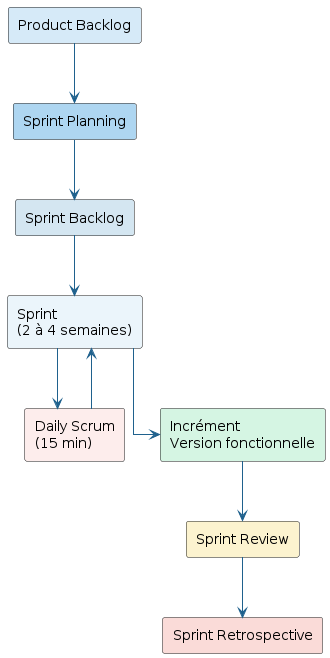
\includegraphics[width=0.5\textwidth]{Figures/Chapitre1/sprintarr.png}
\caption{Diagramme de la méthodologie Scrum}
\label{fig:ch1:scrum}
\end{figure}

\subsection{Langages de modélisation}

Pour la conception du système, le langage UML (Unified Modeling Language) est utilisé. Les principaux
diagrammes utilisés sont :

\begin{itemize}
    \item Diagramme de cas d'utilisation,
    \item Diagramme de classes,
    \item Diagramme de séquence.
\end{itemize}

Ces diagrammes permettent de représenter le fonctionnement du système de manière claire et structurée.

% ─────────────────────────────────────────────────────────────────────────────
\section*{Conclusion}

Ce chapitre a présenté le contexte général du projet et les limites du système existant. L'analyse a
montré la nécessité de développer une solution informatique adaptée. La solution proposée repose sur
une application web de gestion du service après-vente, développée selon la méthodologie Scrum. Le
chapitre suivant sera consacré à la préparation du projet et à la capture des besoins.

\newpage
\pagestyle{fancy}
\lhead{\textsc{Chapitre 2. Préparation du projet}}
\renewcommand{\headrulewidth}{0.5pt}
\renewcommand{\footrulewidth}{0.5pt}
\chapter{Préparation du projet}\setlength{\headheight}{28pt}
\label{ch2}
\thispagestyle{empty}
\minitoc
\newpage

Après avoir présenté le cadre général du projet, nous entamons la phase de préparation du projet
selon la méthodologie Scrum. Cette étape vise à identifier, analyser et modéliser les besoins du
système SAV, ainsi qu'à définir l'organisation du projet, l'environnement de travail et l'architecture
adoptée.

% ─────────────────────────────────────────────────────────────────────────────
\section{Capture des besoins}

\subsection{Spécification des besoins}

\subsubsection{Exigences fonctionnelles}

\begin{table}[H]
\centering
\caption{Exigences fonctionnelles}
\label{tab:ch2:exigences_fonctionnelles}
\begin{tabular}{|p{3.8cm}|p{10.7cm}|}
\hline
\textbf{Module} & \textbf{Description condensée} \\
\hline
Authentification & Connexion par e-mail ou téléphone, contrôle d'accès par rôle (RBAC), déconnexion sécurisée. \\
\hline
Utilisateurs & CRUD des comptes internes (administrateur, technicien) avec désactivation logique et restauration. \\
\hline
Clients & CRUD des fiches clients (société ou personne physique), ville tunisienne, accès portail client. \\
\hline
Équipements & Catalogue global (climatiseur, système de surpression) avec images multiples et image principale. \\
\hline
Affectation & Association équipement–client via \texttt{ClientEquipement} avec date d'achat, date d'installation et localisation. \\
\hline
Contrats & CRUD des contrats couvrant des installations \texttt{ClientEquipement} avec périodicité et statut calculé. \\
\hline
Planning préventif & Génération automatique des interventions préventives lors de la création d'un contrat. \\
\hline
Interventions & Cycle de vie complet (préventives et curatives), affectation technicien avec vérification de disponibilité. \\
\hline
Pannes & Déclaration par le client avec pièces jointes ; conversion en intervention curative par l'administrateur. \\
\hline
Facturation & Génération des factures pour interventions curatives hors contrat (TVA 19\,\%, TND) ; marquage payée. \\
\hline
Tableaux de bord & Dashboard global administrateur, dashboard personnel technicien, espace client différencié. \\
\hline
Historique & Consultation de l'historique des interventions filtrée selon le rôle de l'utilisateur connecté. \\
\hline
\end{tabular}
\end{table}

\subsubsection{Exigences non fonctionnelles}

\begin{table}[H]
\centering
\caption{Exigences non fonctionnelles}
\label{tab:ch2:exigences_nf}
\begin{tabular}{|p{3cm}|p{11.5cm}|}
\hline
\textbf{Exigence} & \textbf{Description} \\
\hline
Sécurité & Authentification obligatoire, contrôle d'accès RBAC, mots de passe chiffrés, session sans stockage en clair. \\
\hline
Performance & Temps de réponse rapide, listes paginées pour limiter le volume de données chargées. \\
\hline
Ergonomie & Interface en français, intuitive, responsive (desktop, tablette, mobile), thèmes clair et sombre. \\
\hline
Maintenabilité & TypeScript avec typage strict, architecture modulaire, composants réutilisables. \\
\hline
Disponibilité & Accessible depuis tout navigateur web moderne sans installation préalable. \\
\hline
Localisation & Monnaie TND, TVA 19\,\%, liste de villes tunisiennes intégrée. \\
\hline
Fiabilité & Validation des données côté client, messages d'erreur explicites. \\
\hline
\end{tabular}
\end{table}

% ─────────────────────────────────────────────────────────────────────────────
\section{Modélisation des besoins}

\subsection{Identification des acteurs}

Le système fait intervenir quatre acteurs ayant des rôles distincts :

\begin{table}[H]
\centering
\caption{Identification des acteurs}
\label{tab:ch2:acteurs}
\begin{tabular}{|p{3.2cm}|p{7.5cm}|}
\hline
\textbf{Acteur} & \textbf{Permissions principales} \\
\hline
\textbf{Administrateur}
  & Gère les utilisateurs, les clients, les équipements, les contrats, les interventions, les factures et le suivi global du système. \\
\hline
\textbf{Technicien}
  & Réalise les interventions, consulte son planning et son historique. \\
\hline
\textbf{Client}
  & Déclare les pannes, consulte ses factures, ses interventions et son historique. \\
\hline
\end{tabular}
\end{table}

\subsection{Identification des cas d'utilisation}

Les associations entre acteurs et cas d'utilisation sont représentées dans le diagramme global.
L'administrateur hérite des fonctionnalités du technicien, tandis que le client dispose d'un accès
limité aux fonctions de déclaration et de consultation.

\subsection{Diagramme de cas d'utilisation global}

\begin{figure}[H]
\centering
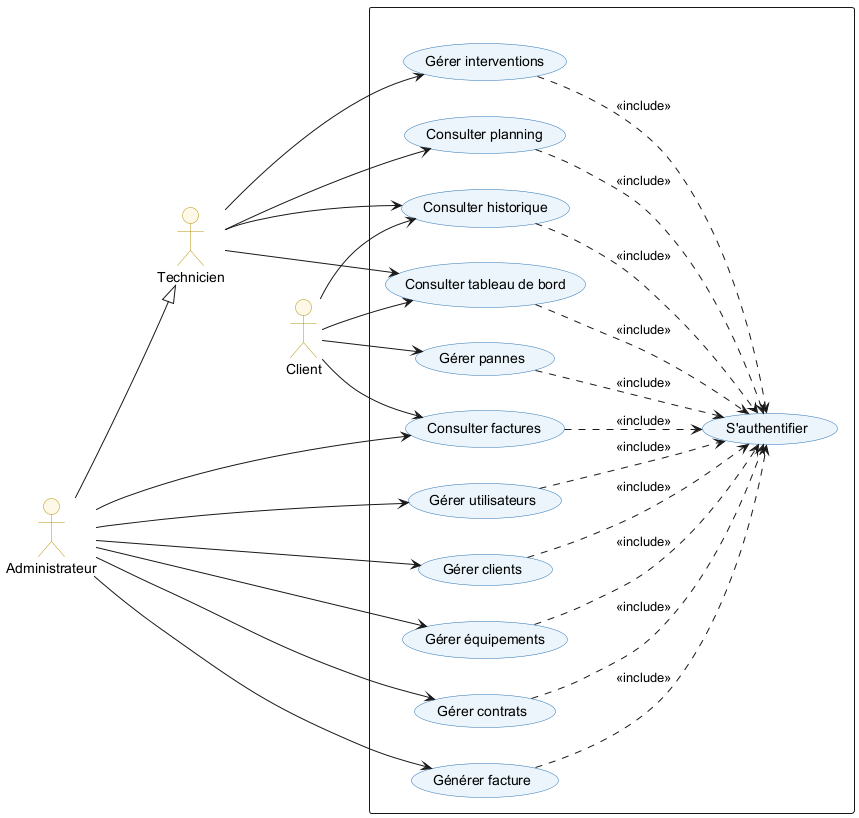
\includegraphics[width=0.7\textwidth]{Figures/Chapitre1/globaluasecase.png}
\caption{Diagramme de cas d'utilisation global}
\label{fig:ch2:usecase_global}
\end{figure}

% ─────────────────────────────────────────────────────────────────────────────
\section{Diagramme de classes global}

Le diagramme de classes global représente la structure générale du système ainsi que les relations
entre les onze entités principales.

\begin{figure}[H]
\centering
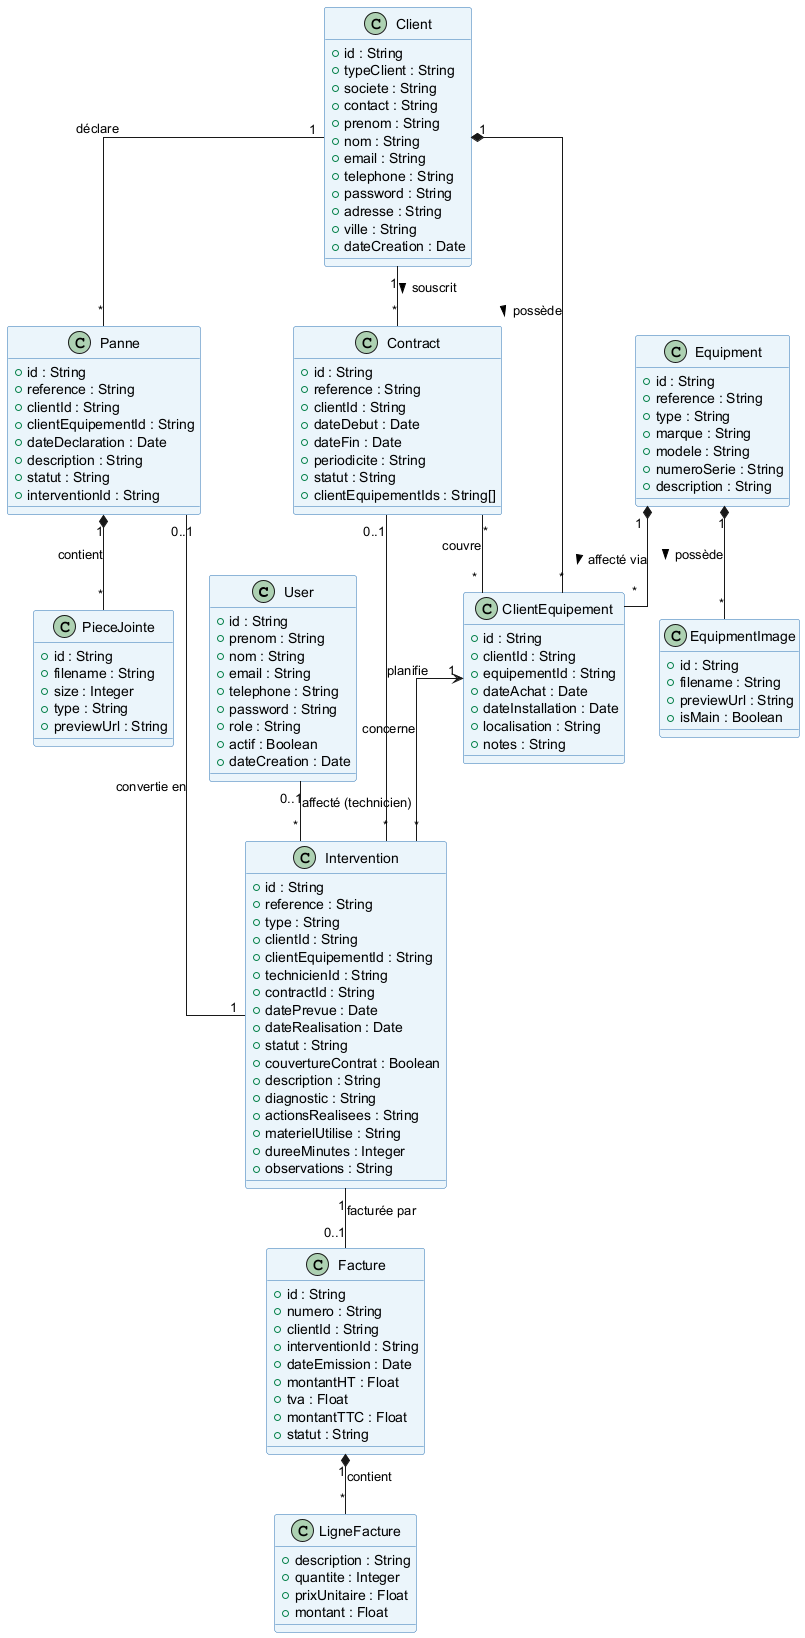
\includegraphics[width=0.8\textwidth]{Figures/Chapitre1/globaldiagramclass.png}
\caption{Diagramme de classes global}
\label{fig:ch2:class_global}
\end{figure}

\textbf{Dictionnaire de données :}

\begin{longtable}{|p{3.2cm}|p{11.3cm}|}
\caption{Dictionnaire de données}
\label{tab:ch2:dictionnaire} \\
\hline
\textbf{Entité} & \textbf{Description} \\
\hline
\endfirsthead
\caption*{Dictionnaire de données (suite)} \\
\hline
\textbf{Entité} & \textbf{Description} \\
\hline
\endhead
\hline
\endfoot
\hline
\endlastfoot
\texttt{User}
  & Utilisateur interne (administrateur ou technicien).
    Attributs : prenom, nom, email, role (\texttt{admin}/\texttt{technician}), actif. \\
\hline
\texttt{Client}
  & Client métier (société ou personne physique).
    Attributs : typeClient, societe, prenom, nom, email, adresse, ville. \\
\hline
\texttt{Equipment}
  & Équipement du catalogue global, indépendant de tout client.
    Attributs : reference, type (\texttt{CLIMATISEUR}/\texttt{SYSTEME\_SURPRESSION}), marque, modele, numeroSerie. \\
\hline
\texttt{EquipmentImage}
  & Image associée à un équipement.
    Attribut notable : isMain (désigne l'image principale). \\
\hline
\texttt{ClientEquipement}
  & Table de jonction \texttt{Client}–\texttt{Equipment} matérialisant une installation.
    Attributs : dateAchat, dateInstallation, localisation (optionnel). \\
\hline
\texttt{Contract}
  & Contrat de maintenance couvrant des installations \texttt{ClientEquipement}.
    Attributs : reference, dateDebut, dateFin, periodicite, statut (\texttt{ACTIF}/\texttt{BIENTOT\_EXPIRE}/\texttt{EXPIRE}). \\
\hline
\texttt{Intervention}
  & Intervention préventive ou curative, sans champ de priorité.
    Attributs : type (\texttt{PREVENTIVE}/\texttt{CURATIVE}), datePrevue, statut (\texttt{PLANIFIEE}/\texttt{EN\_COURS}/\texttt{REALISEE}/\texttt{ANNULEE}), couvertureContrat. \\
\hline
\texttt{Panne}
  & Déclaration de panne par un client, sans champ de priorité.
    Attributs : dateDeclaration, description, statut (\texttt{EN\_ATTENTE}/\texttt{PRISE\_EN\_CHARGE}/\texttt{CONVERTIE}/\texttt{ANNULEE}). \\
\hline
\texttt{PieceJointe}
  & Pièce jointe associée à une panne.
    Attributs : filename, size, type (image, PDF ou audio). \\
\hline
\texttt{Facture}
  & Facture pour une intervention curative réalisée hors contrat.
    Attributs : numero, dateEmission, montantHT, tva (19\,\%), montantTTC, statut (\texttt{PAYEE}/\texttt{IMPAYEE}/\texttt{EN\_ATTENTE}). \\
\hline
\texttt{LigneFacture}
  & Ligne de détail d'une facture.
    Attributs : description, quantite, prixUnitaire, montant. \\
\hline
\end{longtable}

% ─────────────────────────────────────────────────────────────────────────────
\section{Pilotage du projet avec Scrum}

\subsection{Équipe et rôles}

Le projet est organisé selon la méthodologie Scrum. Les rôles principaux sont :

\begin{table}[H]
\centering
\caption{Équipe et rôles Scrum}
\label{tab:ch2:roles}
\begin{tabular}{|p{4.5cm}|p{10cm}|}
\hline
\textbf{Rôle} & \textbf{Description} \\
\hline
\textbf{Product Owner}
  & Définit les besoins fonctionnels du projet et priorise le backlog \\
\hline
\textbf{Scrum Master}
  & Assure le suivi de la méthodologie Scrum et facilite les cérémonies \\
\hline
\textbf{Équipe de développement}
  & Réalise l'analyse, la conception et le développement des fonctionnalités \\
\hline
\end{tabular}
\end{table}

\subsection{Le Backlog du produit}

Le backlog complet comporte 28 user stories. Le tableau suivant présente les user stories représentatives couvrant les principaux modules du système.

\begin{longtable}{|p{1.2cm}|p{7.5cm}|p{2.3cm}|p{1.5cm}|p{1.2cm}|}
\caption{Product Backlog --- sélection représentative (28 user stories au total)}
\label{tab:ch2:backlog} \\
\hline
\textbf{ID} & \textbf{User Story} & \textbf{Acteur} & \textbf{Priorité} & \textbf{Sprint} \\
\hline
\endfirsthead
\caption*{Product Backlog (suite)} \\
\hline
\textbf{ID} & \textbf{User Story} & \textbf{Acteur} & \textbf{Priorité} & \textbf{Sprint} \\
\hline
\endhead
\hline
\endfoot
\hline
\endlastfoot
US-01 & En tant qu'utilisateur, je veux me connecter avec mon e-mail ou mon numéro de téléphone et mon mot de passe. & Tout utilisateur & Haute & S1 \\
\hline
US-04 & Le système restreint automatiquement l'accès aux pages selon le rôle de l'utilisateur. & Système (auto) & Haute & S1 \\
\hline
US-08 & En tant qu'administrateur, je veux affecter un équipement du catalogue à un client via \texttt{ClientEquipement}. & Administrateur & Haute & S1 \\
\hline
US-09 & En tant qu'administrateur, je veux créer un contrat couvrant des installations \texttt{ClientEquipement}. & Administrateur & Haute & S1 \\
\hline
US-11 & En tant qu'administrateur, je veux affecter un technicien disponible à une intervention. & Administrateur & Haute & S2 \\
\hline
US-16 & En tant que client, je veux déclarer une panne avec pièces jointes. & Client & Haute & S2 \\
\hline
US-19 & En tant qu'administrateur, je veux générer une facture pour une intervention curative réalisée hors contrat (TVA 19\,\%, TND). & Administrateur & Haute & S3 \\
\hline
US-25 & En tant qu'administrateur, je veux consulter un tableau de bord global avec KPIs et graphiques. & Administrateur & Haute & S3 \\
\hline
\end{longtable}

\subsection{Planification des sprints}

\begin{longtable}{|p{1.7cm}|p{3.2cm}|p{5.8cm}|p{4cm}|}
\caption{Planification des sprints}
\label{tab:ch2:sprints} \\
\hline
\textbf{Sprint} & \textbf{Objectif} & \textbf{Fonctionnalités couvertes} & \textbf{Entités concernées} \\
\hline
\endfirsthead
\hline
\textbf{Sprint} & \textbf{Objectif} & \textbf{Fonctionnalités couvertes} & \textbf{Entités concernées} \\
\hline
\endhead
\hline
\endfoot
\hline
\endlastfoot
\textbf{Sprint 1}
  & Authentification et référentiel métier
  & Connexion (email ou téléphone), contrôle d'accès RBAC ;
    CRUD utilisateurs (soft-delete), clients et équipements ;
    affectation \texttt{ClientEquipement} ; contrats et planning préventif automatique.
  & \texttt{User}, \texttt{Client}, \texttt{Equipment},
    \texttt{EquipmentImage}, \texttt{ClientEquipement},
    \texttt{Contract} \\
\hline
\textbf{Sprint 2}
  & Gestion des interventions et des pannes
  & Affectation technicien (vérification disponibilité) ;
    démarrage et clôture interventions ;
    déclaration panne avec pièces jointes ;
    conversion panne $\rightarrow$ curative ; vérification couverture contractuelle.
  & \texttt{Intervention}, \texttt{Panne}, \texttt{PieceJointe},
    \texttt{Contract}, \texttt{ClientEquipement} \\
\hline
\textbf{Sprint 3}
  & Facturation, historique et tableaux de bord
  & Génération factures (curative + hors contrat, TVA 19\,\%) ;
    marquage payée ; historique par rôle ;
    dashboards administrateur, technicien et client.
  & \texttt{Facture}, \texttt{LigneFacture}, \texttt{Intervention},
    \texttt{Client}, \texttt{User} \\
\hline
\end{longtable}

% ─────────────────────────────────────────────────────────────────────────────
\section{Environnement de travail}

\subsection{Environnement matériel}

Le développement de l'application a été réalisé avec les équipements suivants :

\begin{table}[H]
\centering
\caption{Environnement matériel}
\label{tab:ch2:materiel}
\begin{tabular}{|p{4cm}|p{10cm}|}
\hline
\textbf{Élément} & \textbf{Caractéristiques} \\
\hline
Machine      & PC Portable \\
\hline
Processeur   & Intel Core i5 \\
\hline
Mémoire RAM  & 8 Go \\
\hline
Stockage     & SSD 512 Go \\
\hline
\end{tabular}
\end{table}

\subsection{Environnement logiciel}

\begin{table}[H]
\centering
\caption{Environnement logiciel}
\label{tab:ch2:logiciel}
\begin{tabular}{|p{4cm}|p{10cm}|}
\hline
\textbf{Outil} & \textbf{Description} \\
\hline
Visual Studio Code & Environnement de développement intégré \\
\hline
Next.js            & Framework Frontend (App Router) \\
\hline
React              & Bibliothèque JavaScript \\
\hline
TypeScript         & Typage statique strict \\
\hline
Tailwind CSS       & Framework CSS utilitaire \\
\hline
Prisma             & ORM pour la base de données \\
\hline
MySQL              & Système de gestion de base de données \\
\hline
\end{tabular}
\end{table}

% ─────────────────────────────────────────────────────────────────────────────
\section{Architecture de l'application}

L'application est construite sur une architecture web en trois couches qui sépare clairement le
frontend, la logique métier et la base de données.

\textbf{Couche présentation (Frontend)} Le frontend de l'application est développé en utilisant
Next.js et React. Cette combinaison permet de créer une interface utilisateur à la fois moderne
et dynamique. Les composants React assurent une séparation claire des responsabilités d'affichage.

\textbf{Couche logique métier (Backend / API)} La couche backend expose des routes API RESTful
implémentées sous forme de contrôleurs. Chaque contrôleur gère la validation des données,
l'exécution de la logique métier et les appels vers la base de données.

\textbf{Couche d'accès aux données (Prisma / MySQL)} L'accès à la base de données est géré
via Prisma ORM. Cette couche exécute les requêtes vers la base de données MySQL et garantit
l'intégrité des données via la gestion des transactions (COMMIT/ROLLBACK).

\begin{figure}[H]
\centering
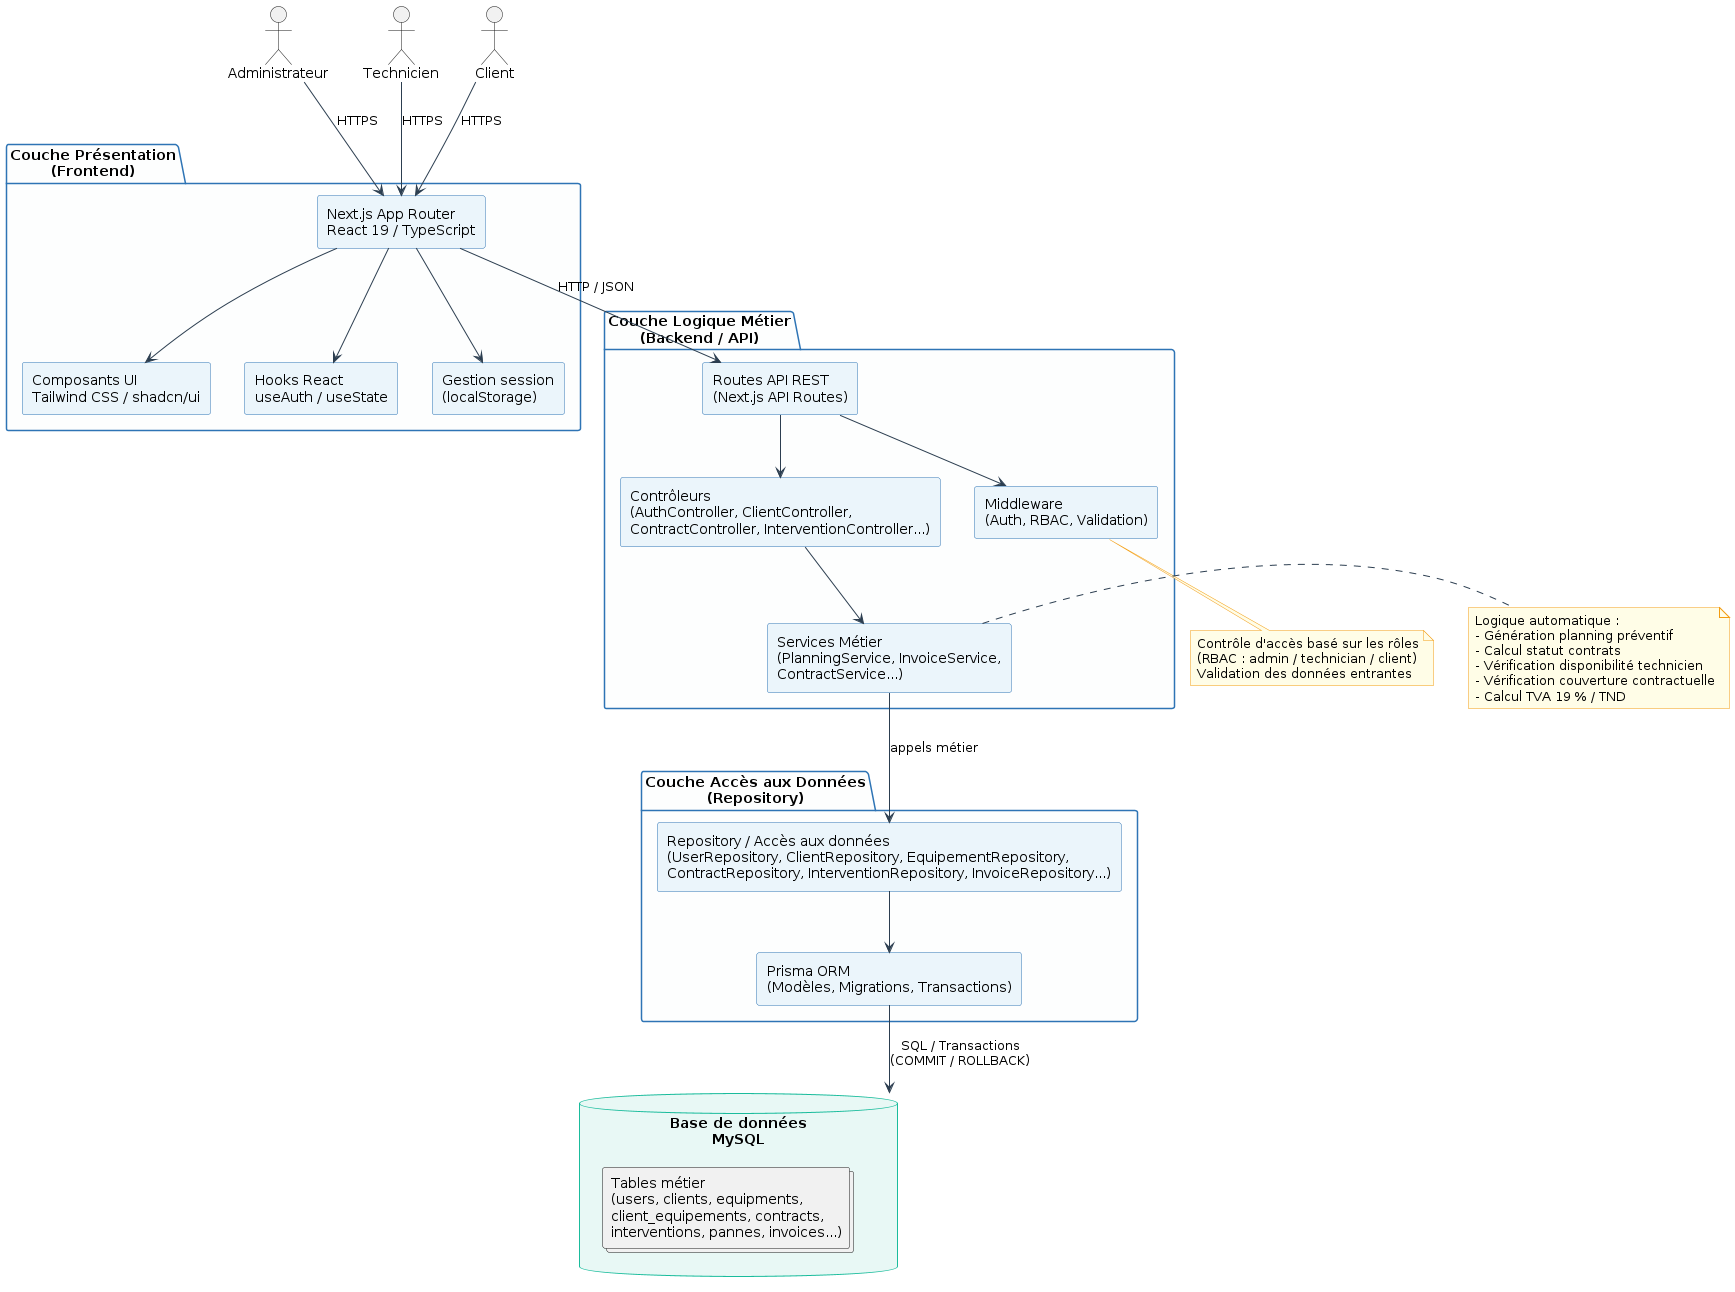
\includegraphics[width=0.8\textwidth]{Figures/Chapitre2/architecture.png}
\caption{Architecture de l'application}
\label{fig:ch2:architecture}
\end{figure}

% ─────────────────────────────────────────────────────────────────────────────
\section*{Conclusion}

Dans ce chapitre, nous avons établi les exigences fonctionnelles et non fonctionnelles de
l'application en précisant leurs règles métier. Nous avons identifié trois acteurs
(Administrateur, Technicien et Client) et représenté leurs interactions à travers 28
User Stories réparties sur 3 sprints. Le schéma de classes global présente les 11 entités du
modèle, incluant l'entité intermédiaire \texttt{ClientEquipement} qui associe les clients aux
équipements du catalogue. Le prochain chapitre traitera du Sprint 1 --- Authentification et
référentiel métier.

\newpage
\pagestyle{fancy}
\lhead{\textsc{Chapitre 3. Sprint 1 --- Authentification et référentiel métier}}
\renewcommand{\headrulewidth}{0.5pt}
\renewcommand{\footrulewidth}{0.5pt}
\chapter{Sprint 1 --- Authentification et référentiel métier}\setlength{\headheight}{28pt}
\label{ch3}
\thispagestyle{empty}
\minitoc
\newpage

Dans le chapitre précédent, nous avons traité de la phase préparatoire du projet ainsi que des
spécifications du système. Ce chapitre aborde le premier sprint du projet, réalisé selon la méthode
Scrum. Ce sprint est essentiel pour le développement de l'application, car il établit les fondations
du système, surtout en ce qui concerne l'authentification des utilisateurs et la gestion des données
cruciales.

Les fonctionnalités développées pendant ce sprint sont principalement axées sur :

\begin{itemize}
    \item L'authentification par e-mail ou numéro de téléphone ;
    \item La gestion des utilisateurs internes avec désactivation logique et restauration ;
    \item La gestion des clients (société ou personne physique) ;
    \item La gestion du catalogue d'équipements avec images multiples ;
    \item L'affectation des équipements aux clients via \texttt{ClientEquipement} ;
    \item La gestion des contrats de maintenance avec génération automatique du planning préventif.
\end{itemize}

% ─────────────────────────────────────────────────────────────────────────────
\section{Backlog du Sprint 1}

\begin{longtable}{|p{1.2cm}|p{7.5cm}|p{2.8cm}|p{1.8cm}|}
\caption{Backlog du Sprint 1}
\label{tab:ch3:backlog_sprint1} \\
\hline
\textbf{ID} & \textbf{User Story} & \textbf{Acteur} & \textbf{Priorité} \\
\hline
\endfirsthead
\caption*{Backlog du Sprint 1 (suite)} \\
\hline
\textbf{ID} & \textbf{User Story} & \textbf{Acteur} & \textbf{Priorité} \\
\hline
\endhead
\hline
\endfoot
\hline
\endlastfoot
US-01 & En tant qu'utilisateur, je veux me connecter avec mon e-mail ou mon numéro de téléphone et mon mot de passe. & Tout utilisateur & Élevée \\
\hline
US-03 & En tant qu'administrateur, je veux gérer les comptes utilisateurs internes (CRUD + désactivation + restauration). & Administrateur & Élevée \\
\hline
US-04 & Le système contrôle automatiquement les accès selon le rôle de l'utilisateur connecté. & Système (auto) & Élevée \\
\hline
US-05 & En tant qu'administrateur, je veux créer une fiche client (société ou personne physique). & Administrateur & Élevée \\
\hline
US-07 & En tant qu'administrateur, je veux ajouter un équipement au catalogue global avec images multiples. & Administrateur & Élevée \\
\hline
US-08 & En tant qu'administrateur, je veux affecter un équipement du catalogue à un client via \texttt{ClientEquipement}. & Administrateur & Élevée \\
\hline
US-09 & En tant qu'administrateur, je veux créer un contrat couvrant des installations \texttt{ClientEquipement}. & Administrateur & Élevée \\
\hline
US-10 & Le système génère automatiquement le planning préventif lors de la création d'un contrat. & Système (auto) & Élevée \\
\hline
\end{longtable}

% ─────────────────────────────────────────────────────────────────────────────
\section{Analyse}

\subsection{Diagramme de cas d'utilisation du Sprint 1}

\begin{figure}[H]
\centering
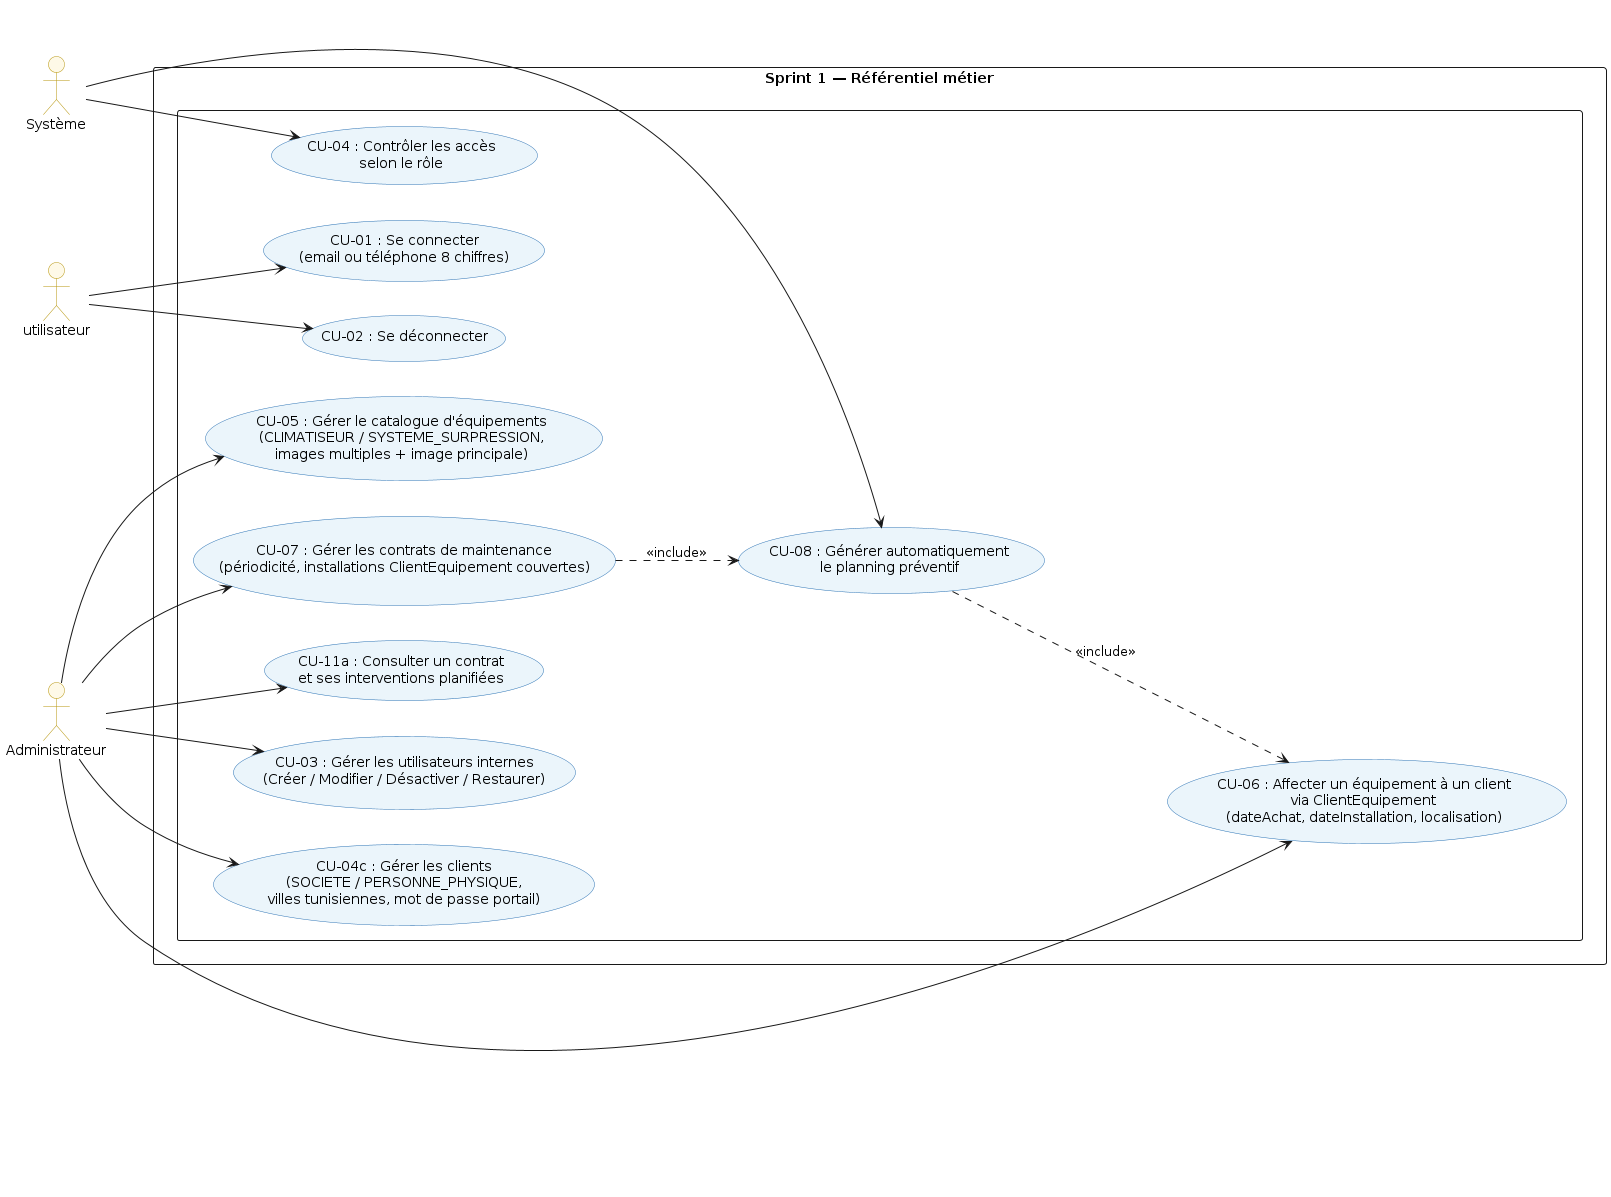
\includegraphics[width=0.70\textwidth]
{Figures/Chapitre3/use_case_sprint1.png}
\caption{Diagramme de cas d'utilisation du Sprint 1}
\label{fig:ch3:usecase_sprint1}
\end{figure}

Acteurs impliqués dans ce sprint :

\textbf{Administrateur} : gestion des utilisateurs, clients, catalogue équipements,
affectation \texttt{ClientEquipement}, contrats.

\textbf{Tout utilisateur} : connexion.

\textit{Comportements automatiques du système :} contrôle d'accès selon le rôle, génération du planning préventif.

\subsection{Description des cas d'utilisation}

\subsubsection{CU-01 : S'authentifier}

\begin{table}[H]
\centering
\caption{CU-01 : S'authentifier}
\label{tab:ch3:cu01}
\begin{tabular}{|p{3.5cm}|p{11cm}|}
\hline
\textbf{Champ} & \textbf{Contenu} \\
\hline
\textbf{Description}
  & Ce cas d'utilisation permet à un utilisateur de s'authentifier dans le système. \\
\hline
\textbf{Acteurs}
  & Administrateur, Technicien, Client \\
\hline
\textbf{Préconditions}
  & L'utilisateur possède un compte valide et actif. \\
\hline
\textbf{Postconditions}
  & L'utilisateur accède à son espace personnel selon son rôle. \\
\hline
\end{tabular}
\end{table}

\textbf{Scénario nominal :}
\begin{enumerate}
    \item L'utilisateur ouvre l'interface de connexion.
    \item Il saisit son identifiant (\textbf{adresse e-mail ou numéro de téléphone à 8 chiffres})
          et son mot de passe.
    \item Le système détecte le type d'identifiant : si l'identifiant contient un « @ »,
          il s'agit d'un e-mail ; sinon, il s'agit d'un numéro de téléphone.
    \item Le système recherche l'utilisateur correspondant dans la base de données.
    \item Le système vérifie le mot de passe.
    \item Le système crée la session et redirige l'utilisateur vers son tableau de bord
          selon son rôle.
\end{enumerate}

\textbf{Scénarios alternatifs :}
\begin{itemize}
    \item Identifiant (e-mail ou téléphone) non reconnu $\rightarrow$ message d'erreur affiché.
    \item Mot de passe incorrect $\rightarrow$ message d'erreur affiché.
    \item Compte inactif (\texttt{actif = false}) $\rightarrow$ accès refusé avec message d'erreur.
\end{itemize}

\subsubsection{CU-03 : Gérer les utilisateurs internes}

\begin{table}[H]
\centering
\caption{CU-03 : Gérer les utilisateurs internes}
\label{tab:ch3:cu03}
\begin{tabular}{|p{3.5cm}|p{11cm}|}
\hline
\textbf{Champ} & \textbf{Contenu} \\
\hline
\textbf{Description}
  & Ce cas d'utilisation permet à l'administrateur de gérer les comptes des utilisateurs
    internes (administrateurs et techniciens). \\
\hline
\textbf{Acteur principal}
  & Administrateur \\
\hline
\textbf{Préconditions}
  & L'administrateur est authentifié. \\
\hline
\textbf{Postconditions}
  & Les modifications sont enregistrées dans la base de données. \\
\hline
\end{tabular}
\end{table}

\textbf{Fonctionnalités :}
\begin{itemize}
    \item Créer un utilisateur interne (prénom, nom, e-mail, téléphone, rôle, mot de passe) ;
    \item Modifier un utilisateur existant ;
    \item Désactiver un utilisateur (soft-delete : \texttt{actif = false}) ;
    \item Restaurer un utilisateur désactivé (\texttt{actif = true}) ;
    \item Consulter la liste des utilisateurs avec filtres.
\end{itemize}

\textbf{Scénario nominal :} Le scénario consiste à saisir les informations requises ou à sélectionner un utilisateur existant, à valider les données côté contrôleur (unicité de l'e-mail, chiffrement du mot de passe), puis à enregistrer la modification en base et à actualiser l'affichage.

\textbf{Règles de gestion :}
\begin{itemize}
    \item Chaque utilisateur interne doit avoir un e-mail unique.
    \item Le mot de passe est chiffré avant stockage.
    \item Un utilisateur désactivé (\texttt{actif = false}) ne peut plus se connecter.
    \item L'action « Restaurer » remet \texttt{actif = true}.
    \item Les comptes clients ne sont pas gérés ici --- ils appartiennent au module Clients.
\end{itemize}

\subsubsection{CU-04 : Gérer les clients}

\begin{table}[H]
\centering
\caption{CU-04 : Gérer les clients}
\label{tab:ch3:cu04}
\begin{tabular}{|p{3.5cm}|p{11cm}|}
\hline
\textbf{Champ} & \textbf{Contenu} \\
\hline
\textbf{Description}
  & Ce cas d'utilisation permet à l'administrateur de gérer les fiches clients. \\
\hline
\textbf{Acteur principal}
  & Administrateur \\
\hline
\textbf{Préconditions}
  & L'administrateur est authentifié. \\
\hline
\textbf{Postconditions}
  & Les modifications sont enregistrées dans la base de données. \\
\hline
\end{tabular}
\end{table}

\textbf{Fonctionnalités :}
\begin{itemize}
    \item Créer un client de type \textbf{société} (champs : raison sociale societe, nom du contact)
          ou \textbf{personne physique} (champs : prenom, nom) ;
    \item Renseigner e-mail, téléphone, adresse, ville (liste tunisienne), mot de passe portail ;
    \item Modifier et supprimer un client ;
    \item Consulter la liste avec filtres.
\end{itemize}

\textbf{Règles de gestion :}
\begin{itemize}
    \item Le type \texttt{SOCIETE} requiert le champ societe (raison sociale).
    \item Le type \texttt{PERSONNE\_PHYSIQUE} requiert les champs prenom et nom.
    \item L'e-mail doit être unique dans le système.
    \item Chaque client dispose d'un mot de passe pour accéder au portail client.
\end{itemize}

\subsubsection{CU-05 : Gérer le catalogue d'équipements}

\begin{table}[H]
\centering
\caption{CU-05 : Gérer le catalogue d'équipements}
\label{tab:ch3:cu05}
\begin{tabular}{|p{3.5cm}|p{11cm}|}
\hline
\textbf{Champ} & \textbf{Contenu} \\
\hline
\textbf{Description}
  & Ce cas d'utilisation permet à l'administrateur de gérer le catalogue global d'équipements,
    indépendant de tout client. \\
\hline
\textbf{Acteur principal}
  & Administrateur \\
\hline
\textbf{Préconditions}
  & L'administrateur est authentifié. \\
\hline
\textbf{Postconditions}
  & L'équipement est enregistré dans le catalogue. \\
\hline
\end{tabular}
\end{table}

\textbf{Fonctionnalités :}
\begin{itemize}
    \item Créer un équipement avec : référence, type (\texttt{CLIMATISEUR} ou
          \texttt{SYSTEME\_SURPRESSION}), marque, modèle, numéro de série, description ;
    \item Ajouter plusieurs images (\texttt{EquipmentImage}) dont une image principale
          (\texttt{isMain = true}) ;
    \item Modifier et supprimer un équipement ;
    \item Consulter le catalogue avec filtres par type et marque.
\end{itemize}

\textbf{Règles de gestion :}
\begin{itemize}
    \item Le catalogue est global : un équipement n'appartient pas à un client spécifique.
    \item Le numéro de série est unique.
    \item Une seule image est désignée comme image principale.
\end{itemize}

\subsubsection{CU-06 : Affecter un équipement à un client (\texttt{ClientEquipement})}

\begin{table}[H]
\centering
\caption{CU-06 : Affecter un équipement à un client}
\label{tab:ch3:cu06}
\begin{tabular}{|p{3.5cm}|p{11cm}|}
\hline
\textbf{Champ} & \textbf{Contenu} \\
\hline
\textbf{Description}
  & Ce cas d'utilisation permet à l'administrateur de créer un enregistrement
    \texttt{ClientEquipement} qui matérialise l'installation d'un équipement du catalogue
    chez un client. \\
\hline
\textbf{Acteur principal}
  & Administrateur \\
\hline
\textbf{Préconditions}
  & L'administrateur est authentifié ; le client existe ; l'équipement existe dans le catalogue. \\
\hline
\textbf{Postconditions}
  & Un enregistrement \texttt{ClientEquipement} est créé en base de données. \\
\hline
\end{tabular}
\end{table}

\textbf{Scénario nominal :} L'administrateur sélectionne l'équipement et le client, renseigne la date d'installation et valide ; le contrôleur vérifie l'existence des deux entités et l'absence de doublon avant d'enregistrer le \texttt{ClientEquipement}.

\textbf{Règles de gestion :}
\begin{itemize}
    \item La date d'installation est obligatoire. La localisation est facultative.
    \item Un même équipement peut être affecté à plusieurs clients différents
          (via des enregistrements \texttt{ClientEquipement} distincts).
    \item L'affectation ne modifie pas le catalogue global.
\end{itemize}

\subsubsection{CU-07 : Gérer les contrats de maintenance}

\begin{table}[H]
\centering
\caption{CU-07 : Gérer les contrats de maintenance}
\label{tab:ch3:cu07}
\begin{tabular}{|p{3.5cm}|p{11cm}|}
\hline
\textbf{Champ} & \textbf{Contenu} \\
\hline
\textbf{Description}
  & Ce cas d'utilisation permet à l'administrateur de créer un contrat de maintenance
    couvrant des installations \texttt{ClientEquipement}. \\
\hline
\textbf{Acteur principal}
  & Administrateur \\
\hline
\textbf{Préconditions}
  & L'administrateur est authentifié ; le client existe ; des enregistrements
    \texttt{ClientEquipement} existent pour ce client. \\
\hline
\textbf{Postconditions}
  & Le contrat est enregistré en base ; les interventions préventives sont générées
    automatiquement par le Système. \\
\hline
\end{tabular}
\end{table}

\textbf{Scénario nominal :} L'administrateur saisit les informations du contrat (client, dates, périodicité, installations \texttt{ClientEquipement} couvertes) ; le contrôleur vérifie la cohérence des dates et l'appartenance des installations au client, enregistre le contrat dans une transaction et déclenche la génération automatique du planning préventif.

\textbf{Scénarios alternatifs :} En cas d'erreur (dates invalides, installations non rattachées au client ou échec base de données), l'opération est interrompue, la transaction est annulée et un message explicite est affiché.

\textbf{Règles de gestion :}
\begin{itemize}
    \item Un contrat couvre des installations \texttt{ClientEquipement}, et non des équipements
          du catalogue directement.
    \item Le statut est calculé dynamiquement : \texttt{ACTIF} si fin > aujourd'hui + 30 jours ;
          \texttt{BIENTOT\_EXPIRE} si fin entre aujourd'hui et aujourd'hui + 30 jours ;
          \texttt{EXPIRE} si fin < aujourd'hui.
    \item La génération du planning est automatique et ne requiert aucune action manuelle
          de l'administrateur.
\end{itemize}

\subsubsection{CU-08 : Générer automatiquement le planning préventif}

\begin{table}[H]
\centering
\caption{CU-08 : Générer automatiquement le planning préventif}
\label{tab:ch3:cu08}
\begin{tabular}{|p{3.5cm}|p{11cm}|}
\hline
\textbf{Champ} & \textbf{Contenu} \\
\hline
\textbf{Description}
  & Ce cas d'utilisation décrit le traitement automatique déclenché par le système lors
    de la sauvegarde d'un contrat. \\
\hline
\textbf{Déclencheur}
  & Comportement automatique du système \\
\hline
\textbf{Préconditions}
  & Un contrat valide vient d'être enregistré avec ses \texttt{clientEquipementIds[]},
    ses dates et sa périodicité. \\
\hline
\textbf{Postconditions}
  & Les interventions préventives sont créées en base de données pour toute la durée
    du contrat. \\
\hline
\end{tabular}
\end{table}

\textbf{Scénario nominal :} Le système calcule les dates d'intervention selon la périodicité et les installations couvertes, puis génère les interventions préventives dans une transaction unique.

\textbf{Règles de gestion :}
\begin{itemize}
    \item La génération est automatique : elle est déclenchée par la sauvegarde du contrat,
          non par une action manuelle.
    \item Une intervention préventive est générée pour chaque couple
          (date, \texttt{ClientEquipement} couvert).
    \item Périodicités : mensuelle (12/an), trimestrielle (4/an), semestrielle (2/an),
          annuelle (1/an).
\end{itemize}

% ─────────────────────────────────────────────────────────────────────────────
\section{Conception}

\subsection{Diagramme de classes du Sprint 1}

\begin{figure}[H]
\centering
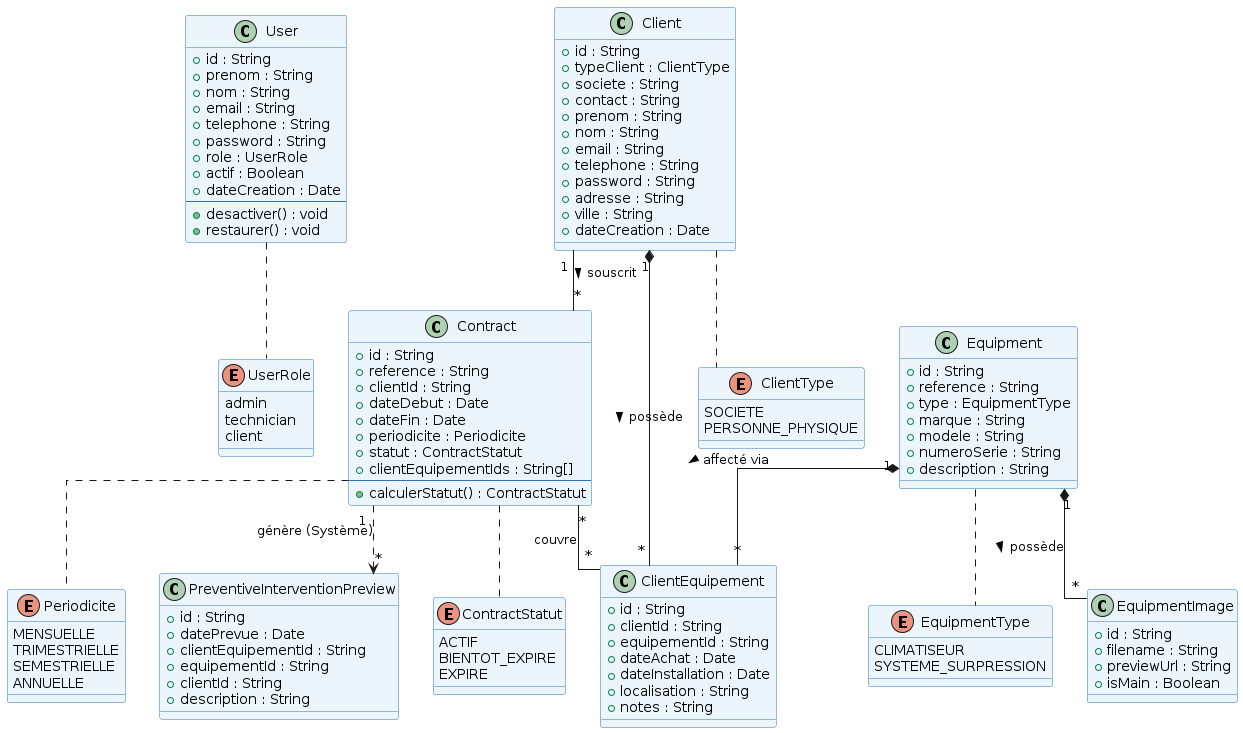
\includegraphics[width=0.70\textwidth]{Figures/Chapitre3/class_diagram_sprint1.png}
\caption{Diagramme de classes du Sprint 1}
\label{fig:ch3:class_sprint1}
\end{figure}

Les entités impliquées dans ce sprint sont : \texttt{User}, \texttt{Client}, \texttt{Equipment},
\texttt{EquipmentImage}, \texttt{ClientEquipement}, \texttt{Contract}, \texttt{Intervention}
(préventive générée automatiquement).

\subsection{Diagrammes de séquence}

\subsubsection{Diagramme de séquence : Connexion (email ou téléphone)}

\begin{figure}[H]
\centering
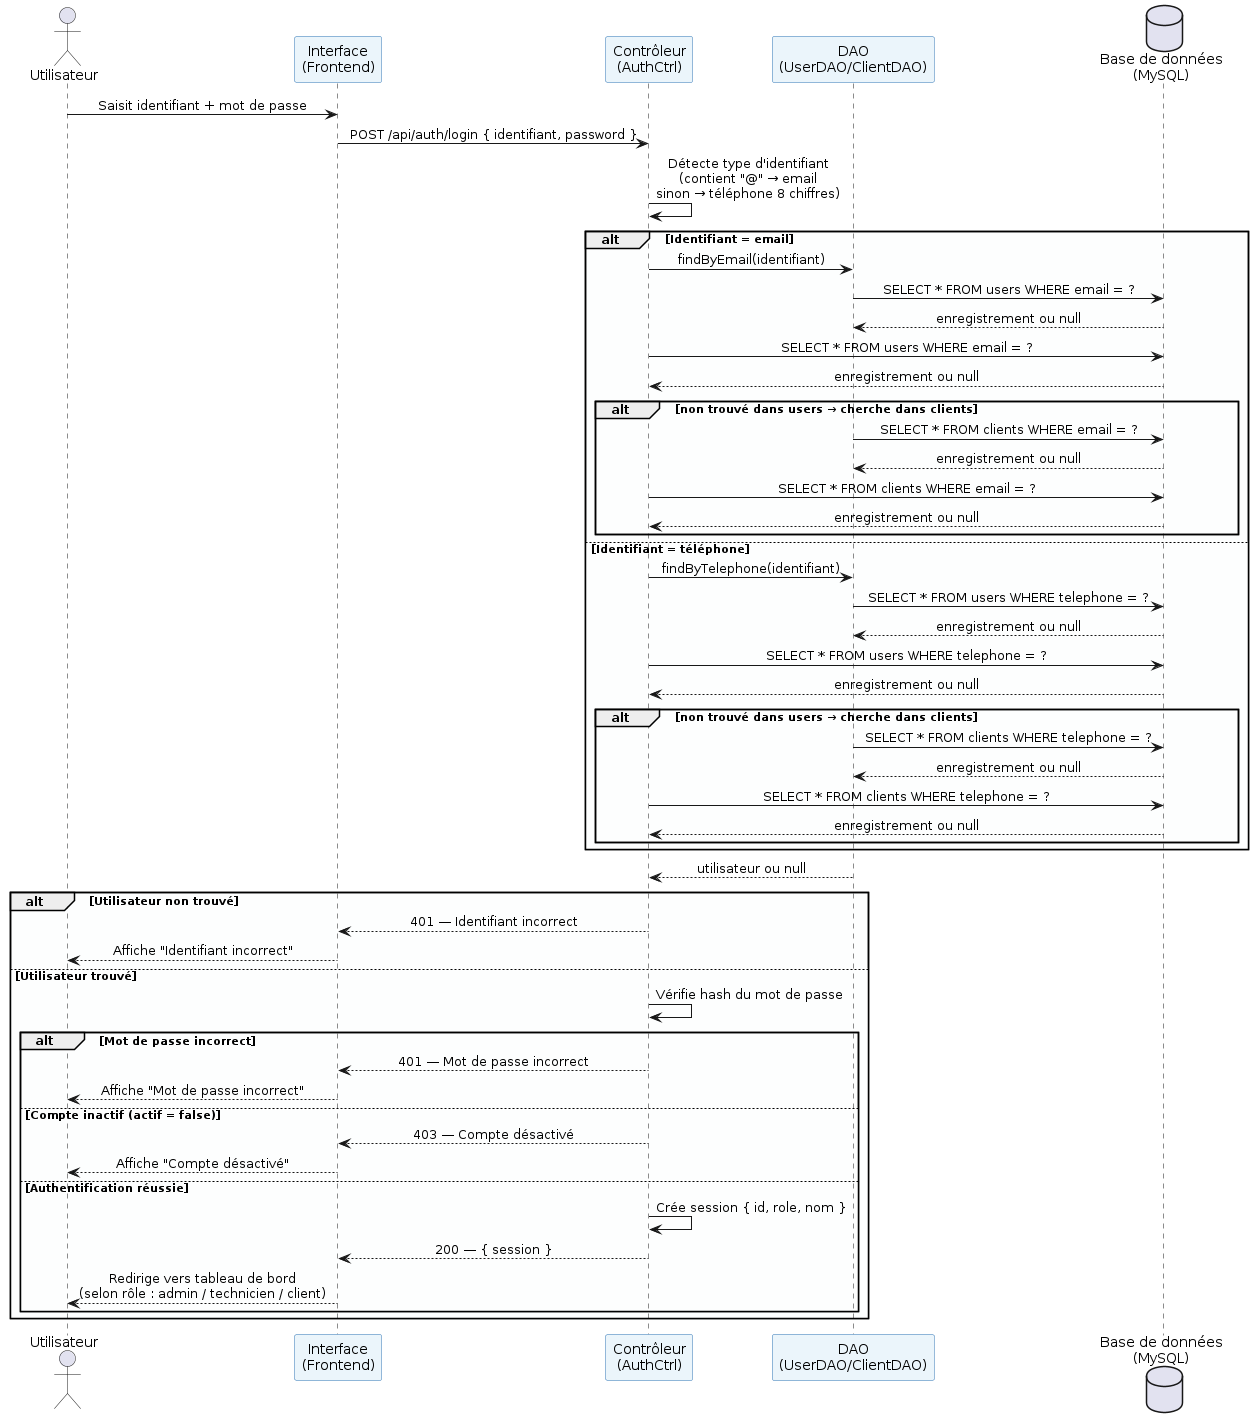
\includegraphics[width=0.70\textwidth]{Figures/Chapitre3/seq_connexion_sprint1.png}
\caption{Diagramme de séquence : Connexion}
\label{fig:ch3:seq_connexion}
\end{figure}

\subsubsection{Diagramme de séquence : Ajout équipement et gestion des images}

\begin{figure}[H]
\centering
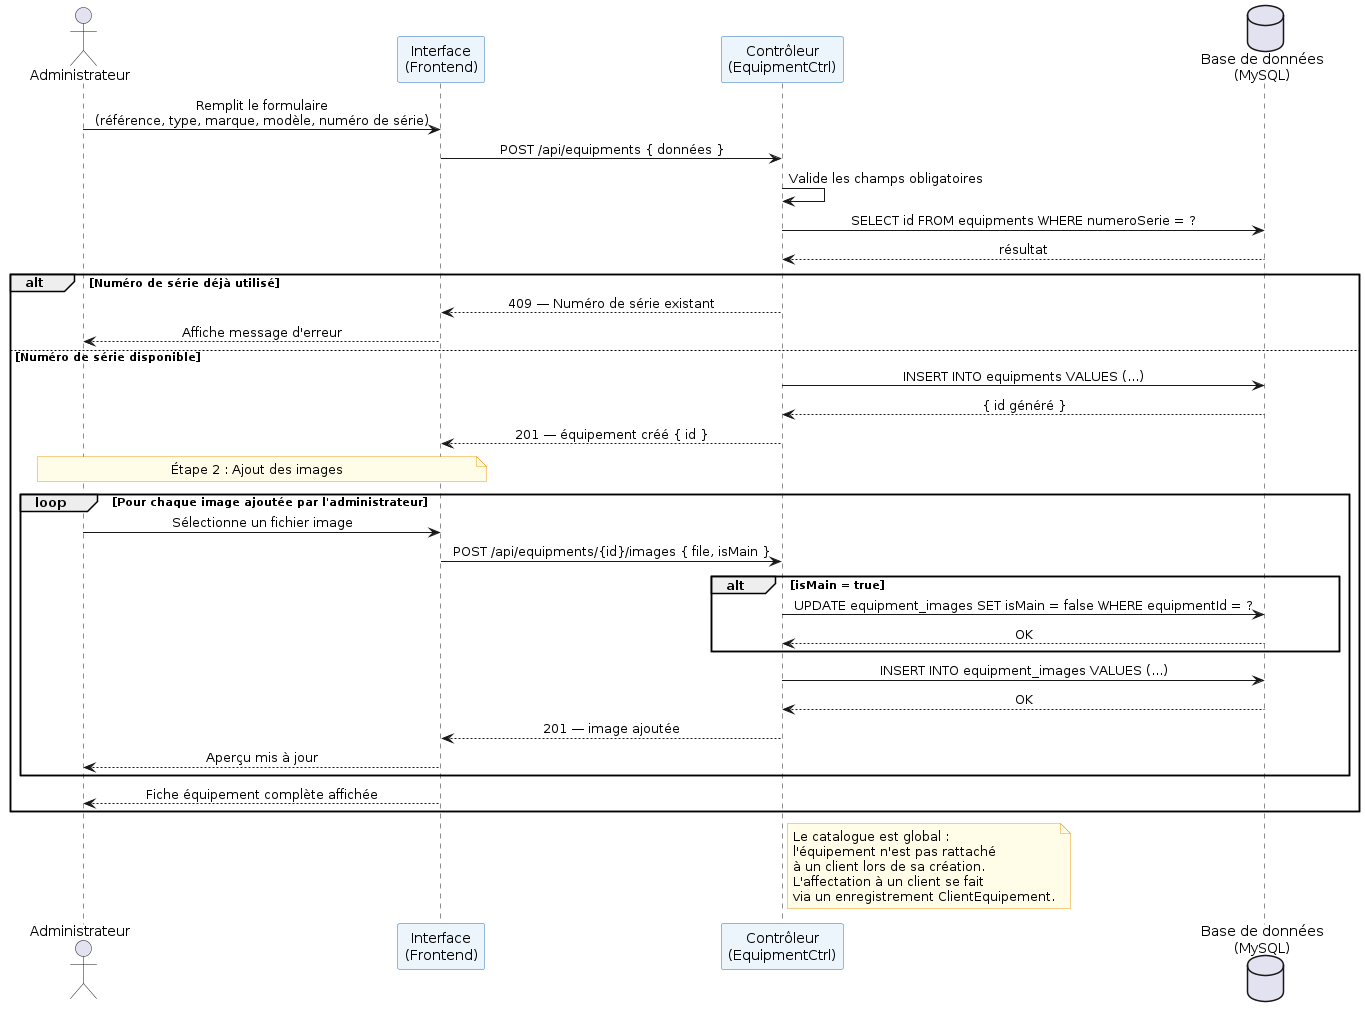
\includegraphics[width=0.70\textwidth]{Figures/Chapitre3/seq_ajoutequip_sprint1.png}
\caption{Diagramme de séquence : Ajout équipement et gestion des images}
\label{fig:ch3:seq_ajout_equipement}
\end{figure}

% ─────────────────────────────────────────────────────────────────────────────
\section{Réalisation}

\begin{figure}[H]
    \centering
    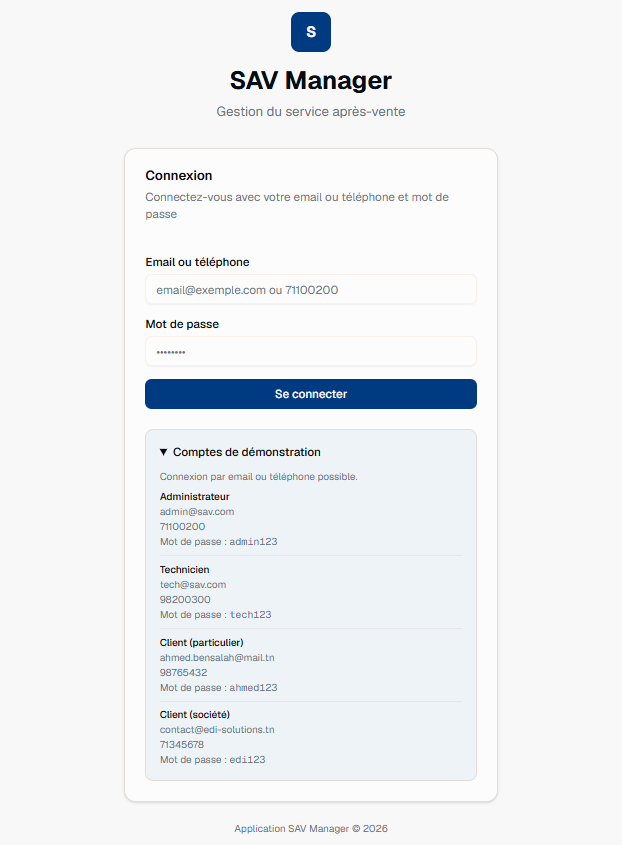
\includegraphics[width=0.74\textwidth]{Figures/Chapitre3/login.png}
    \caption{Capture d'écran : interface de connexion}
    \label{fig:ch3:login}
\end{figure}

\begin{figure}[H]
    \centering
    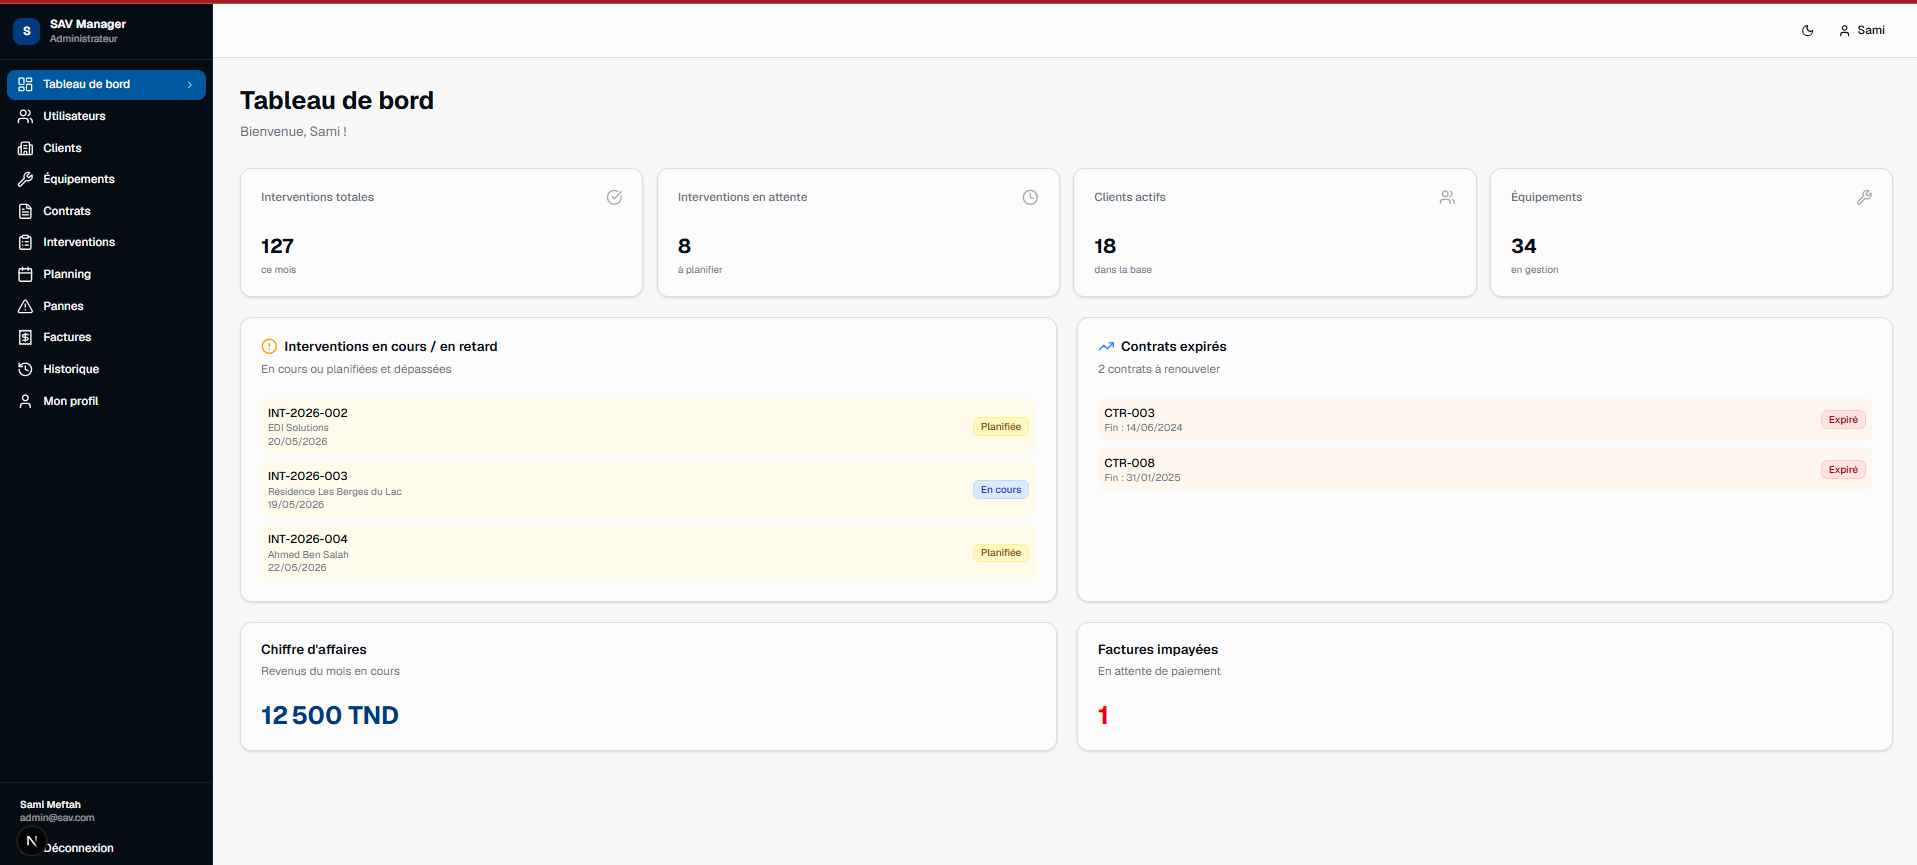
\includegraphics[width=0.74\textwidth]{Figures/Chapitre3/dashboardadmin.png}
    \caption{Capture d'écran : tableau de bord administrateur}
    \label{fig:ch3:dashboard_admin}
\end{figure}

\begin{figure}[H]
    \centering
    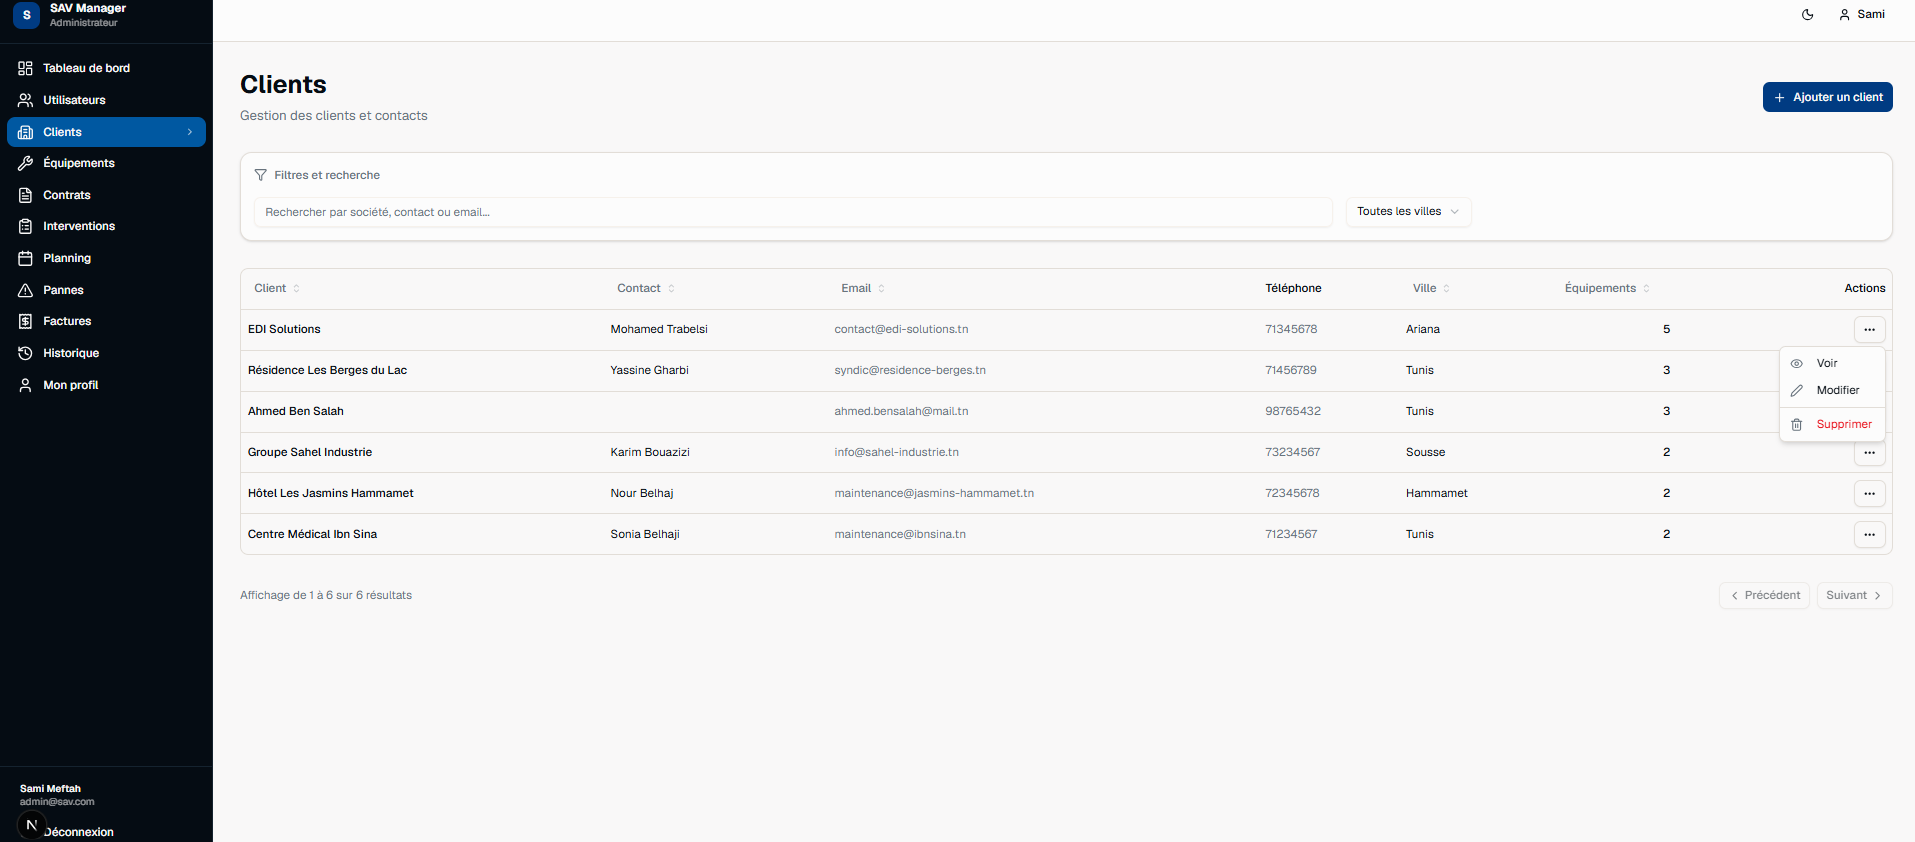
\includegraphics[width=0.74\textwidth]{Figures/Chapitre3/gestclient.png}
    \caption{Capture d'écran : gestion des clients}
    \label{fig:ch3:gestion_clients}
\end{figure}

\begin{figure}[H]
    \centering
    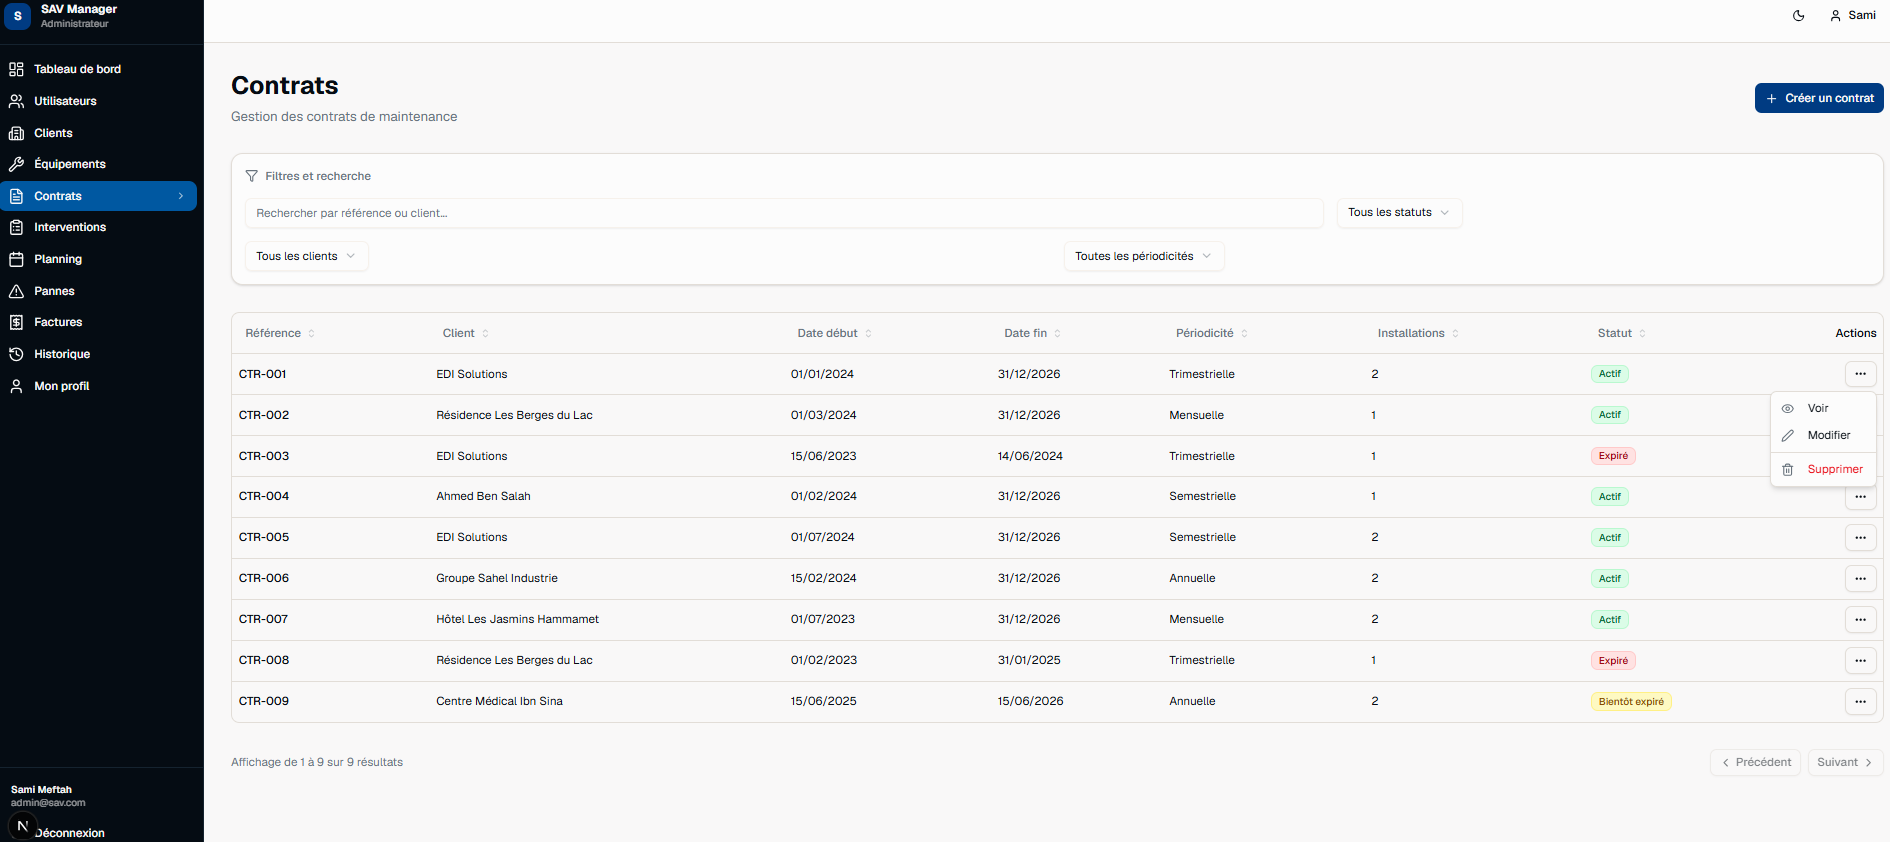
\includegraphics[width=0.74\textwidth]{Figures/Chapitre3/gestcontrat.png}
    \caption{Capture d'écran : gestion des contrats}
    \label{fig:ch3:gestion_contrats}
\end{figure}

% ─────────────────────────────────────────────────────────────────────────────
\section*{Conclusion}

Ce sprint a permis de mettre en place les fondations du système : l'authentification sécurisée
par e-mail ou téléphone, la gestion des référentiels métier (utilisateurs, clients, catalogue
équipements avec images, affectation \texttt{ClientEquipement}), la gestion des contrats et la
génération automatique du planning préventif par le Système. Le chapitre suivant présente le
Sprint 2 dédié à la gestion des interventions et des pannes.

\newpage
\pagestyle{fancy}
\lhead{\textsc{Chapitre 4. Sprint 2 --- Gestion des interventions}}
\renewcommand{\headrulewidth}{0.5pt}
\renewcommand{\footrulewidth}{0.5pt}
\chapter{Sprint 2 --- Gestion des interventions}\setlength{\headheight}{28pt}
\label{ch4}
\thispagestyle{empty}
\minitoc
\newpage

Suite à l'implémentation des fonctionnalités fondamentales du système lors du Sprint 1, ce deuxième
sprint se concentre sur la gestion des interventions préventives et correctives, la déclaration des
pannes et le calendrier des techniciens. Ce sprint constitue le noyau fonctionnel du système SAV.

Les caractéristiques élaborées au cours de ce sprint portent principalement sur :

\begin{itemize}
    \item La vérification du calendrier sur une base hebdomadaire et mensuelle ;
    \item La répartition des techniciens avec contrôle de disponibilité ;
    \item Le début et la fin des interventions par les techniciens ;
    \item Les clients peuvent déclarer des pannes avec plusieurs pièces jointes ;
    \item La gestion et la transformation des pannes en actions correctives ;
    \item L'automatisation de la vérification de la couverture contractuelle lors de la clôture.
\end{itemize}

% ─────────────────────────────────────────────────────────────────────────────
\section{Backlog du Sprint 2}

\begin{longtable}{|p{1.2cm}|p{7.5cm}|p{2.8cm}|p{1.8cm}|}
\caption{Backlog du Sprint 2 --- US-11 à US-20}
\label{tab:ch4:backlog_sprint2} \\
\hline
\textbf{ID} & \textbf{User Story} & \textbf{Acteur} & \textbf{Priorité} \\
\hline
\endfirsthead
\caption*{Backlog du Sprint 2 (suite)} \\
\hline
\textbf{ID} & \textbf{User Story} & \textbf{Acteur} & \textbf{Priorité} \\
\hline
\endhead
\hline
\endfoot
\hline
\endlastfoot
US-11 & En tant qu'administrateur, je veux affecter un technicien disponible à une intervention. & Administrateur & Élevée \\
\hline
US-12 & En tant qu'administrateur/technicien, je veux consulter le planning en vue hebdomadaire ou mensuelle. & Admin / Technicien & Élevée \\
\hline
US-13 & En tant que technicien, je veux démarrer une intervention assignée. & Technicien & Élevée \\
\hline
US-14 & En tant que technicien, je veux clôturer une intervention préventive. & Technicien & Élevée \\
\hline
US-15 & En tant que technicien, je veux clôturer une intervention curative avec vérification de la couverture contractuelle. & Technicien & Élevée \\
\hline
US-16 & En tant que client, je veux déclarer une panne sur l'un de mes équipements, avec pièces jointes. & Client & Élevée \\
\hline
US-17 & En tant qu'administrateur, je veux prendre en charge une panne et la convertir en intervention curative. & Administrateur & Élevée \\
\hline
US-18 & En tant qu'administrateur, je veux créer directement une intervention curative. & Administrateur & Élevée \\
\hline
\end{longtable}

% ─────────────────────────────────────────────────────────────────────────────
\section{Analyse}

\subsection{Diagramme de cas d'utilisation du Sprint 2}

\begin{figure}[H]
\centering
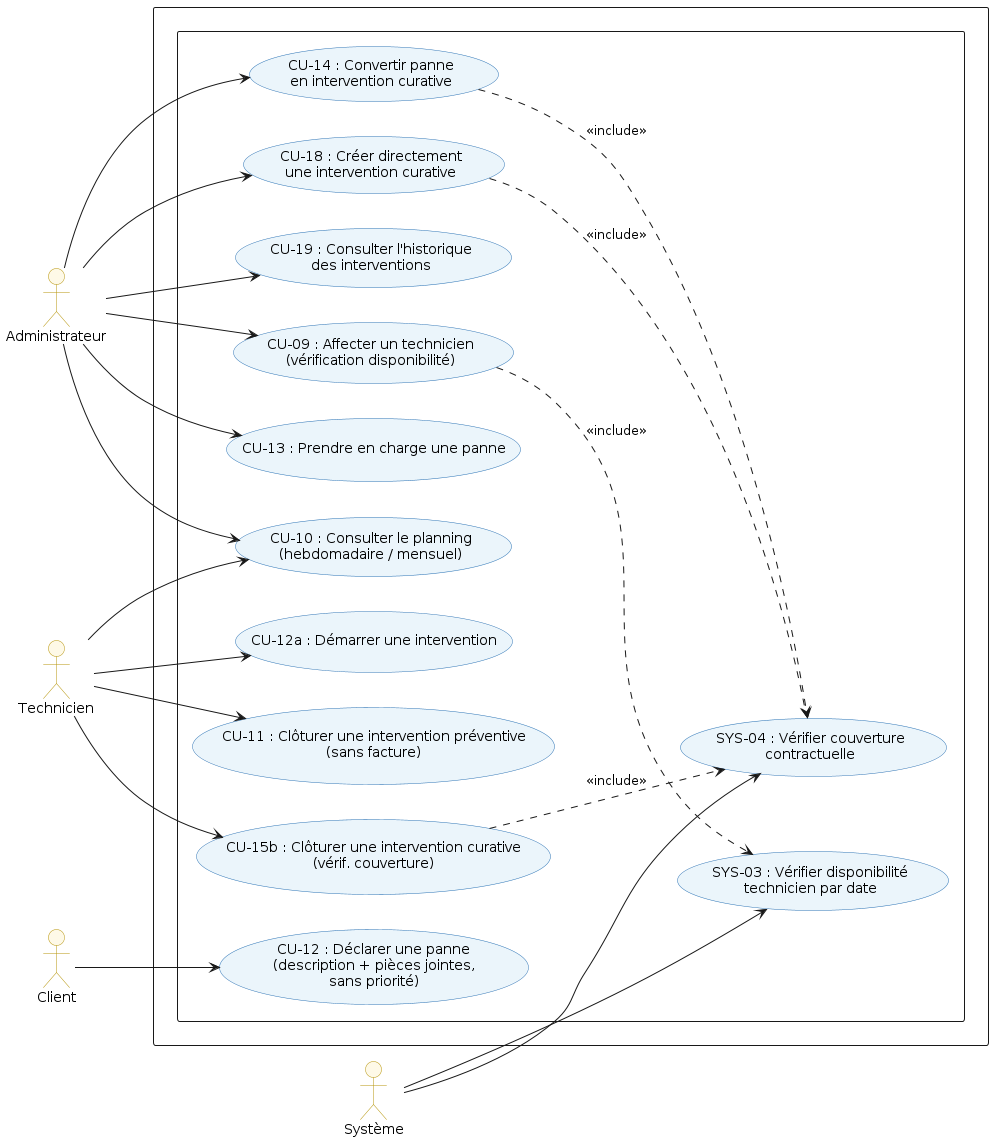
\includegraphics[width=0.70\textwidth]{Figures/Chapitre4/use_case_sprint2.png}
\caption{Diagramme de cas d'utilisation du Sprint 2}
\label{fig:ch4:usecase_sprint2}
\end{figure}

Les acteurs impliqués dans ce sprint sont :

\textbf{Administrateur} : affectation technicien, création intervention curative, prise en charge
et conversion panne, consultation planning global, historique.

\textbf{Technicien} : consultation planning personnel, démarrage et clôture d'interventions.

\textbf{Client} : déclaration de panne avec pièces jointes.

\textit{Comportements automatiques du système :} vérification de disponibilité du technicien, vérification de la couverture contractuelle.

\subsection{Description des cas d'utilisation}

\subsubsection{CU-09 : Affecter un technicien à une intervention}

\begin{table}[H]
\centering
\caption{CU-09 : Affecter un technicien à une intervention}
\label{tab:ch4:cu09}
\begin{tabular}{|p{3.5cm}|p{11cm}|}
\hline
\textbf{Champ} & \textbf{Contenu} \\
\hline
\textbf{Description}
  & Ce cas d'utilisation permet à l'administrateur d'affecter un technicien disponible
    à une intervention planifiée. \\
\hline
\textbf{Acteur principal}
  & Administrateur \\
\hline
\textbf{Préconditions}
  & L'administrateur est authentifié ; l'intervention existe ; le technicien possède
    un compte actif. \\
\hline
\textbf{Postconditions}
  & Le technicien est affecté ; le statut de l'intervention devient \texttt{PLANIFIEE} ;
    l'intervention apparaît dans le planning du technicien. \\
\hline
\end{tabular}
\end{table}

\textbf{Scénario nominal :} L'administrateur sélectionne l'intervention et le technicien à affecter ; le système vérifie l'existence, le statut et la disponibilité du technicien avant d'enregistrer l'affectation.

\textbf{Règles de gestion :}
\begin{itemize}
    \item Seuls les techniciens actifs peuvent être affectés.
    \item \textbf{Un technicien ne peut pas être affecté à deux interventions prévues à la même date.}
    \item L'affectation met automatiquement le statut de l'intervention à \texttt{PLANIFIEE}.
    \item Toute condition invalide (intervention introuvable, technicien inactif, indisponibilité à la date ou erreur technique) interrompt l'opération avec un message explicite.
\end{itemize}

\subsubsection{CU-10 : Consulter le planning}

\begin{table}[H]
\centering
\caption{CU-10 : Consulter le planning}
\label{tab:ch4:cu10}
\begin{tabular}{|p{3.5cm}|p{11cm}|}
\hline
\textbf{Champ} & \textbf{Contenu} \\
\hline
\textbf{Description}
  & Permet de consulter les interventions programmées sous forme de calendrier. \\
\hline
\textbf{Acteurs}
  & Administrateur, Technicien \\
\hline
\textbf{Préconditions}
  & Des interventions planifiées existent. \\
\hline
\textbf{Postconditions}
  & Le planning est affiché selon le rôle. \\
\hline
\end{tabular}
\end{table}

\textbf{Scénario nominal :} L'utilisateur ouvre le module Planning ; le système filtre les interventions selon le rôle et les affiche sous forme de calendrier hebdomadaire ou mensuel.

\textbf{Règles de gestion :}
\begin{itemize}
    \item Le technicien ne voit que les interventions dont il est l'affectataire.
    \item Des filtres sont disponibles pour l'administrateur (type, statut, technicien).
\end{itemize}

\subsubsection{CU-11 : Clôturer une intervention préventive}

\begin{table}[H]
\centering
\caption{CU-11 : Clôturer une intervention préventive}
\label{tab:ch4:cu11}
\begin{tabular}{|p{3.5cm}|p{11cm}|}
\hline
\textbf{Champ} & \textbf{Contenu} \\
\hline
\textbf{Description}
  & Permet au technicien de clôturer une intervention préventive réalisée. \\
\hline
\textbf{Acteur principal}
  & Technicien \\
\hline
\textbf{Préconditions}
  & Le technicien est authentifié et affecté à l'intervention ; le statut est
    \texttt{PLANIFIEE} ou \texttt{EN\_COURS}. \\
\hline
\textbf{Postconditions}
  & Le statut passe à \texttt{REALISEE} ; aucune facture n'est générée. \\
\hline
\end{tabular}
\end{table}

\textbf{Scénario nominal :} Le technicien saisit le compte rendu, les actions réalisées, le matériel utilisé et la durée ; le contrôleur vérifie l'affectation et le statut, puis met à jour l'intervention à \texttt{REALISEE}.

\textbf{Règles de gestion :}
\begin{itemize}
    \item Seul le technicien affecté peut clôturer l'intervention.
    \item \textbf{Une intervention préventive ne génère jamais de facture.}
    \item La durée est saisie en minutes.
\end{itemize}

\subsubsection{CU-12 : Déclarer une panne}

\begin{table}[H]
\centering
\caption{CU-12 : Déclarer une panne}
\label{tab:ch4:cu12}
\begin{tabular}{|p{3.5cm}|p{11cm}|}
\hline
\textbf{Champ} & \textbf{Contenu} \\
\hline
\textbf{Description}
  & Ce cas d'utilisation permet au client de signaler une panne sur l'un de ses équipements. \\
\hline
\textbf{Acteur principal}
  & Client \\
\hline
\textbf{Préconditions}
  & Le client est authentifié ; il possède au moins un équipement affecté. \\
\hline
\textbf{Postconditions}
  & La panne est enregistrée avec le statut \texttt{EN\_ATTENTE}. \\
\hline
\end{tabular}
\end{table}

\textbf{Scénario nominal :} Le client sélectionne un équipement affecté, saisit la description obligatoire et joint éventuellement des pièces jointes ; le système valide l'appartenance de l'équipement, enregistre la panne et lui attribue le statut \texttt{EN\_ATTENTE}.

\textbf{Scénarios alternatifs :}
\begin{itemize}
    \item SA1 : Description manquante $\rightarrow$ validation échoue ;
          message « Description obligatoire ».
    \item SA2 : Équipement non rattaché au client $\rightarrow$ erreur
          « Équipement introuvable ».
\end{itemize}

\textbf{Règles de gestion :}
\begin{itemize}
    \item La description est obligatoire.
    \item \textbf{Aucun champ de priorité n'est présent.}
    \item Les pièces jointes sont de type image, PDF ou audio.
    \item La panne est créée avec le statut \texttt{EN\_ATTENTE}.
\end{itemize}

\subsubsection{CU-13 : Prendre en charge une panne}

\begin{table}[H]
\centering
\caption{CU-13 : Prendre en charge une panne}
\label{tab:ch4:cu13}
\begin{tabular}{|p{3.5cm}|p{11cm}|}
\hline
\textbf{Champ} & \textbf{Contenu} \\
\hline
\textbf{Description}
  & Permet à l'administrateur de prendre en charge une panne déclarée. \\
\hline
\textbf{Acteur principal}
  & Administrateur \\
\hline
\textbf{Préconditions}
  & Une panne a été déclarée avec le statut \texttt{EN\_ATTENTE}. \\
\hline
\textbf{Postconditions}
  & Le statut de la panne passe à \texttt{PRISE\_EN\_CHARGE}. \\
\hline
\end{tabular}
\end{table}

\textbf{Scénario nominal :} L'administrateur sélectionne une panne \texttt{EN\_ATTENTE} et déclenche la prise en charge ; le statut est mis à jour à \texttt{PRISE\_EN\_CHARGE}.

\subsubsection{CU-14 : Convertir une panne en intervention curative}

\begin{table}[H]
\centering
\caption{CU-14 : Convertir une panne en intervention curative}
\label{tab:ch4:cu14}
\begin{tabular}{|p{3.5cm}|p{11cm}|}
\hline
\textbf{Champ} & \textbf{Contenu} \\
\hline
\textbf{Description}
  & Permet à l'administrateur de convertir une panne en intervention curative afin
    d'organiser le traitement technique. \\
\hline
\textbf{Acteur principal}
  & Administrateur \\
\hline
\textbf{Préconditions}
  & Une panne est en statut \texttt{EN\_ATTENTE} ou \texttt{PRISE\_EN\_CHARGE}. \\
\hline
\textbf{Postconditions}
  & Une intervention curative est créée ; la panne passe au statut \texttt{CONVERTIE}. \\
\hline
\end{tabular}
\end{table}

\textbf{Scénario nominal :} L'administrateur sélectionne la panne à convertir, saisit la date prévue et affecte optionnellement un technicien disponible ; le système crée l'intervention curative liée à la panne, vérifie automatiquement la couverture contractuelle, renseigne \texttt{couvertureContrat} et fait passer la panne au statut \texttt{CONVERTIE}.

\textbf{Règles de gestion :}
\begin{itemize}
    \item \textbf{Aucun champ de priorité n'est associé à l'intervention curative créée.}
    \item La couverture contractuelle est vérifiée automatiquement par le Système : si un contrat actif couvre l'installation \texttt{ClientEquipement} à la date de l'intervention, \texttt{couvertureContrat} = true ; sinon false.
    \item Si un technicien est affecté, la disponibilité est vérifiée.
\end{itemize}

% ─────────────────────────────────────────────────────────────────────────────
\section{Conception}

\subsection{Diagramme de classes du Sprint 2}

\begin{figure}[H]
\centering
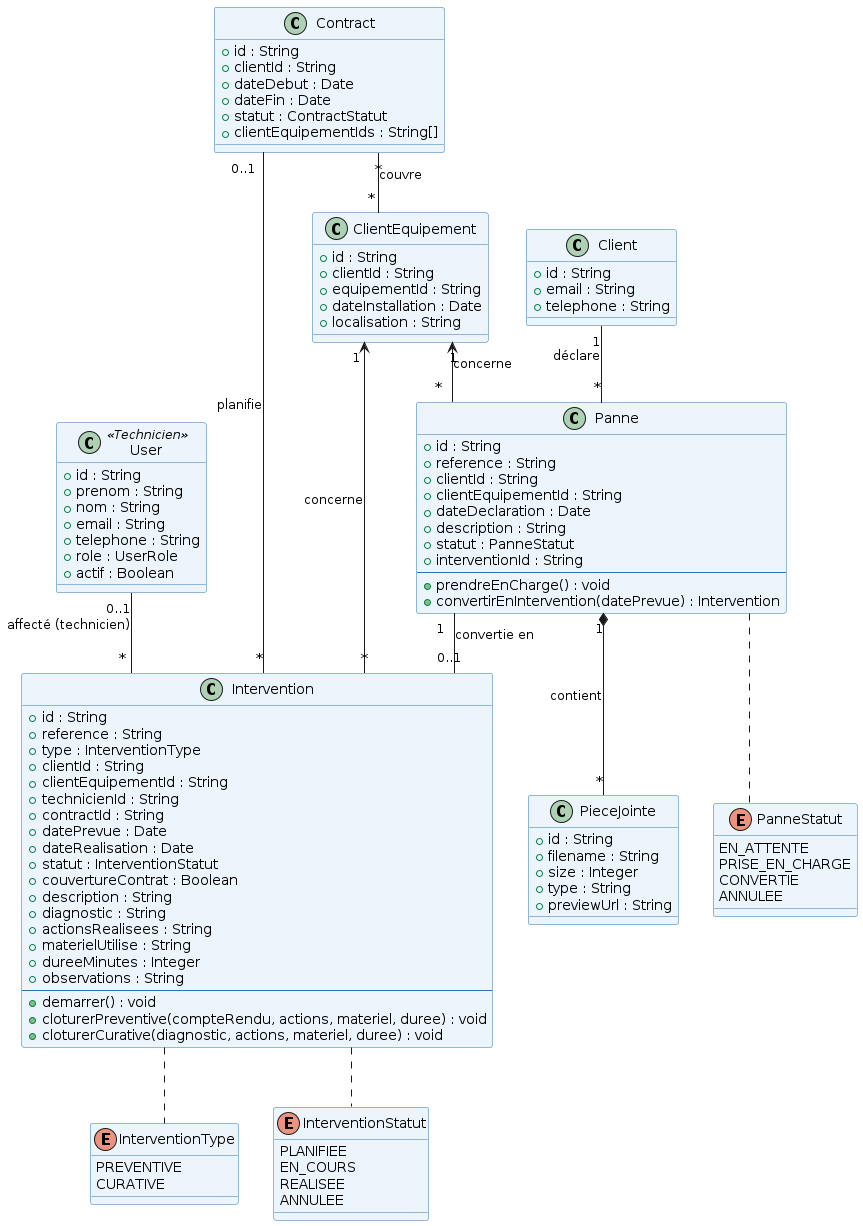
\includegraphics[width=0.70\textwidth]{Figures/Chapitre4/class_diagram_sprint2.png}
\caption{Diagramme de classes du Sprint 2}
\label{fig:ch4:class_sprint2}
\end{figure}

Les entités impliquées dans ce sprint sont : \texttt{Intervention}, \texttt{Panne},
\texttt{PieceJointe}, \texttt{Contract}, \texttt{ClientEquipement}, \texttt{User} (technicien).

\subsection{Diagrammes de séquence}

La génération du planning préventif est déclenchée lors de la création du contrat, comme présenté dans le Sprint 1.

\subsubsection{Diagramme de séquence : Clôture intervention curative et vérification couverture}

\begin{figure}[H]
\centering
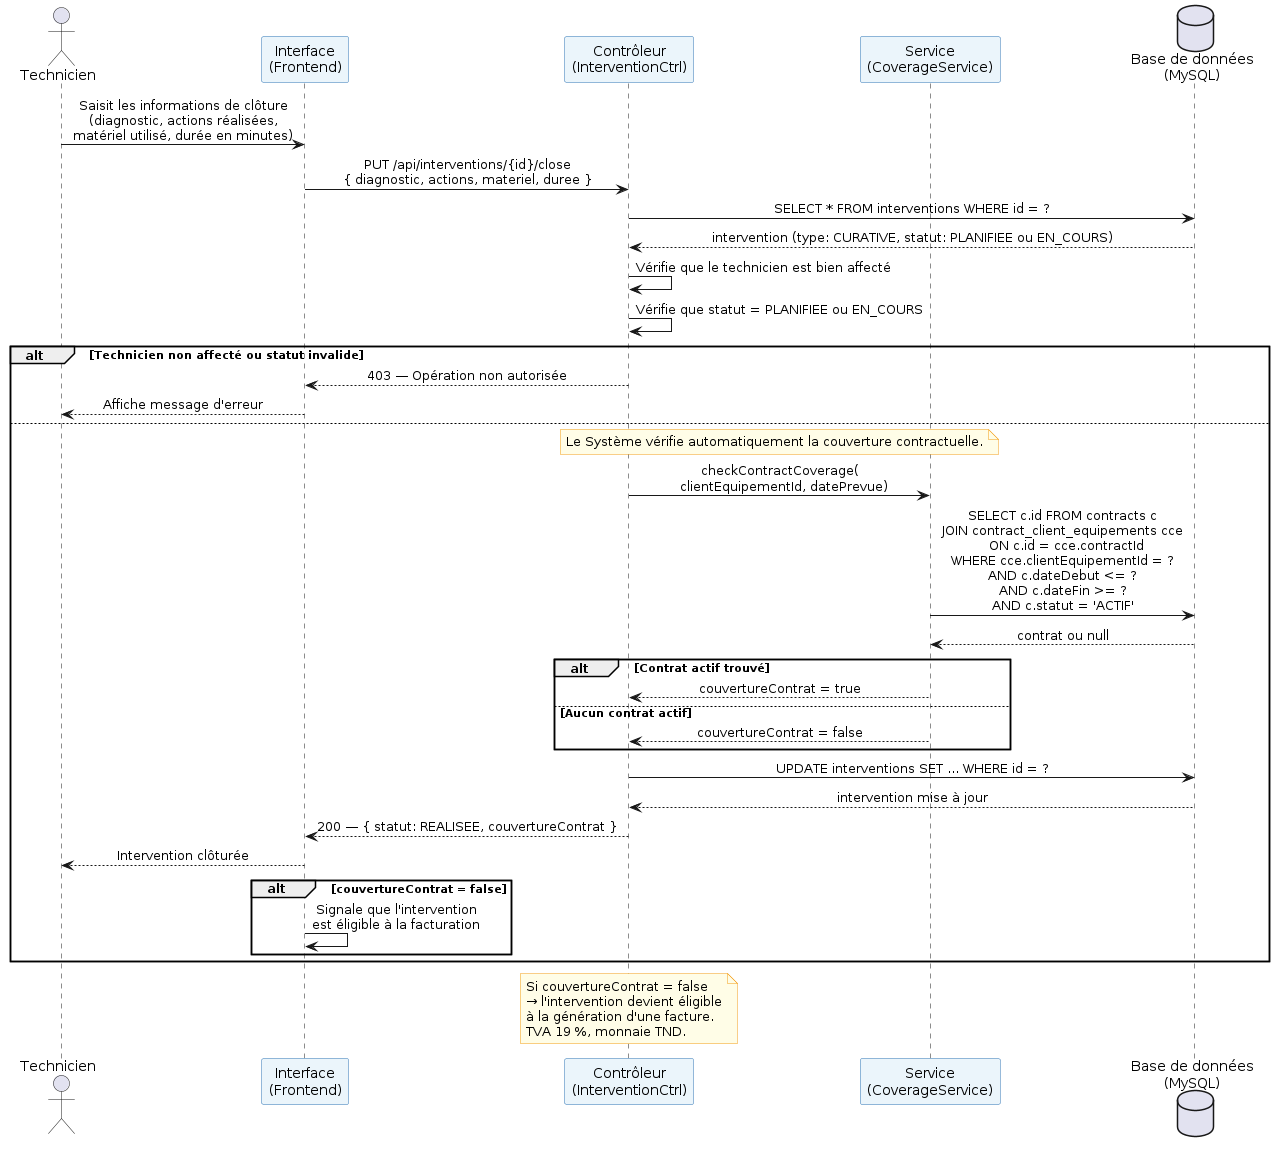
\includegraphics[width=0.70\textwidth]{Figures/Chapitre4/seq_cloturercurative_sprint2.png}
\caption{Diagramme de séquence : Clôture intervention curative et vérification couverture}
\label{fig:ch4:seq_cloture_curative}
\end{figure}

% ─────────────────────────────────────────────────────────────────────────────
\section{Réalisation}

\begin{figure}[H]
    \centering
    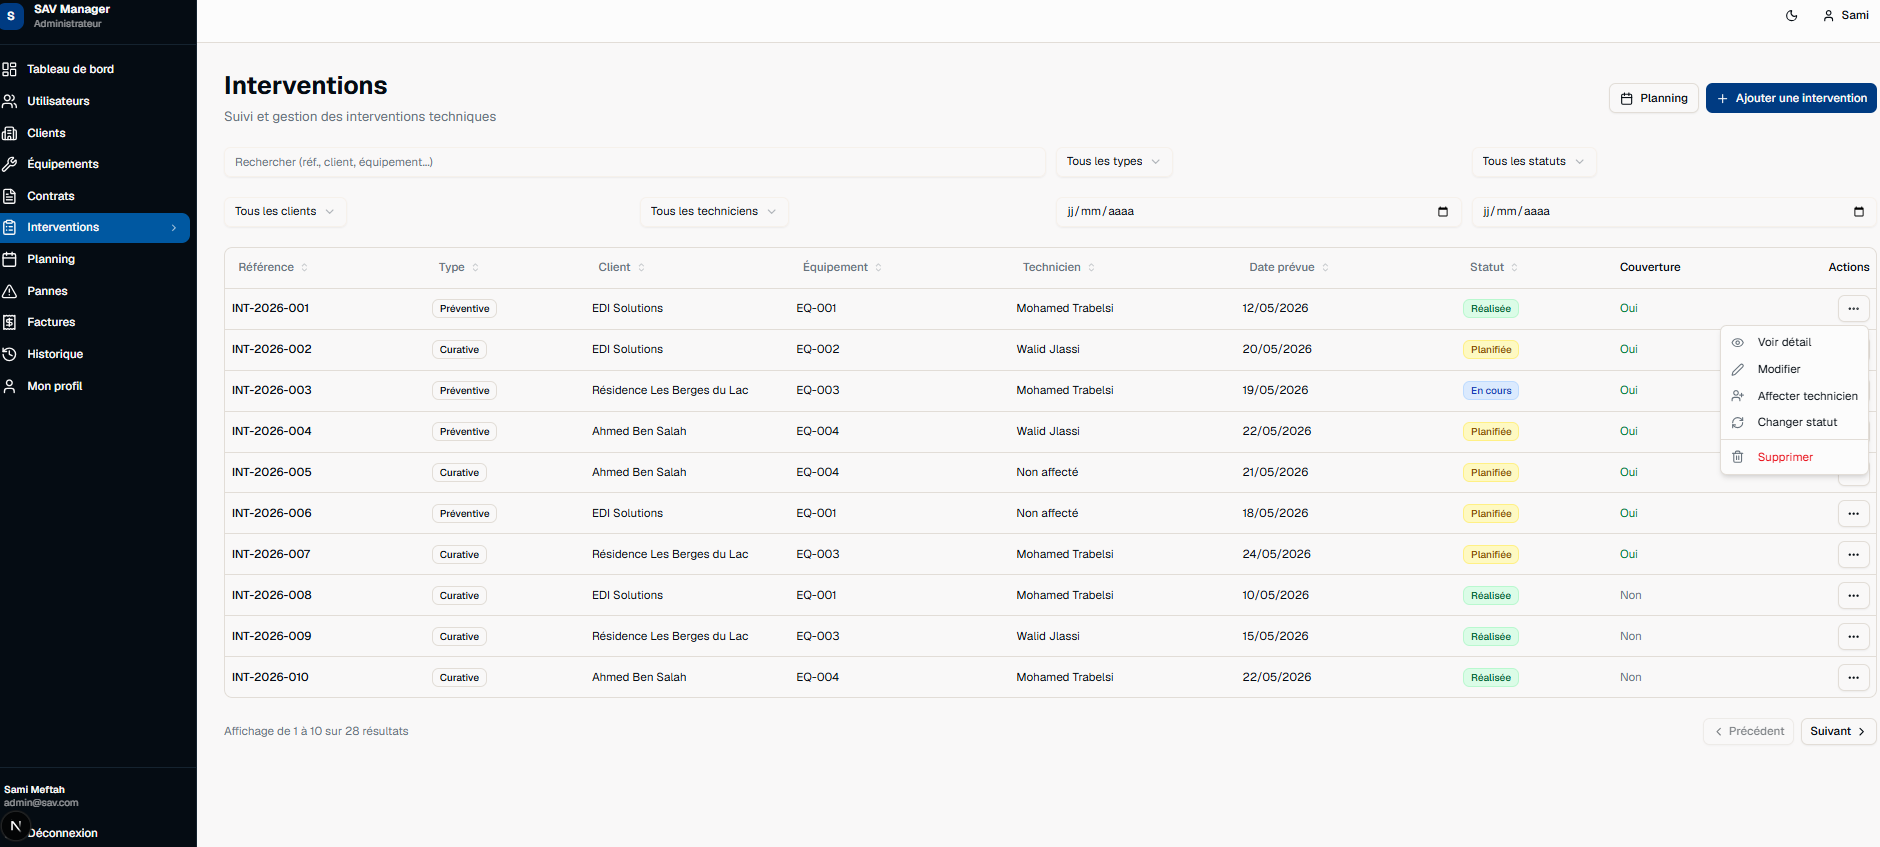
\includegraphics[width=0.74\textwidth]{Figures/Chapitre4/gestintervention.png}
    \caption{Capture d'écran : gestion des interventions}
    \label{fig:ch4:realisation_sprint2_interventions}
\end{figure}

\begin{figure}[H]
    \centering
    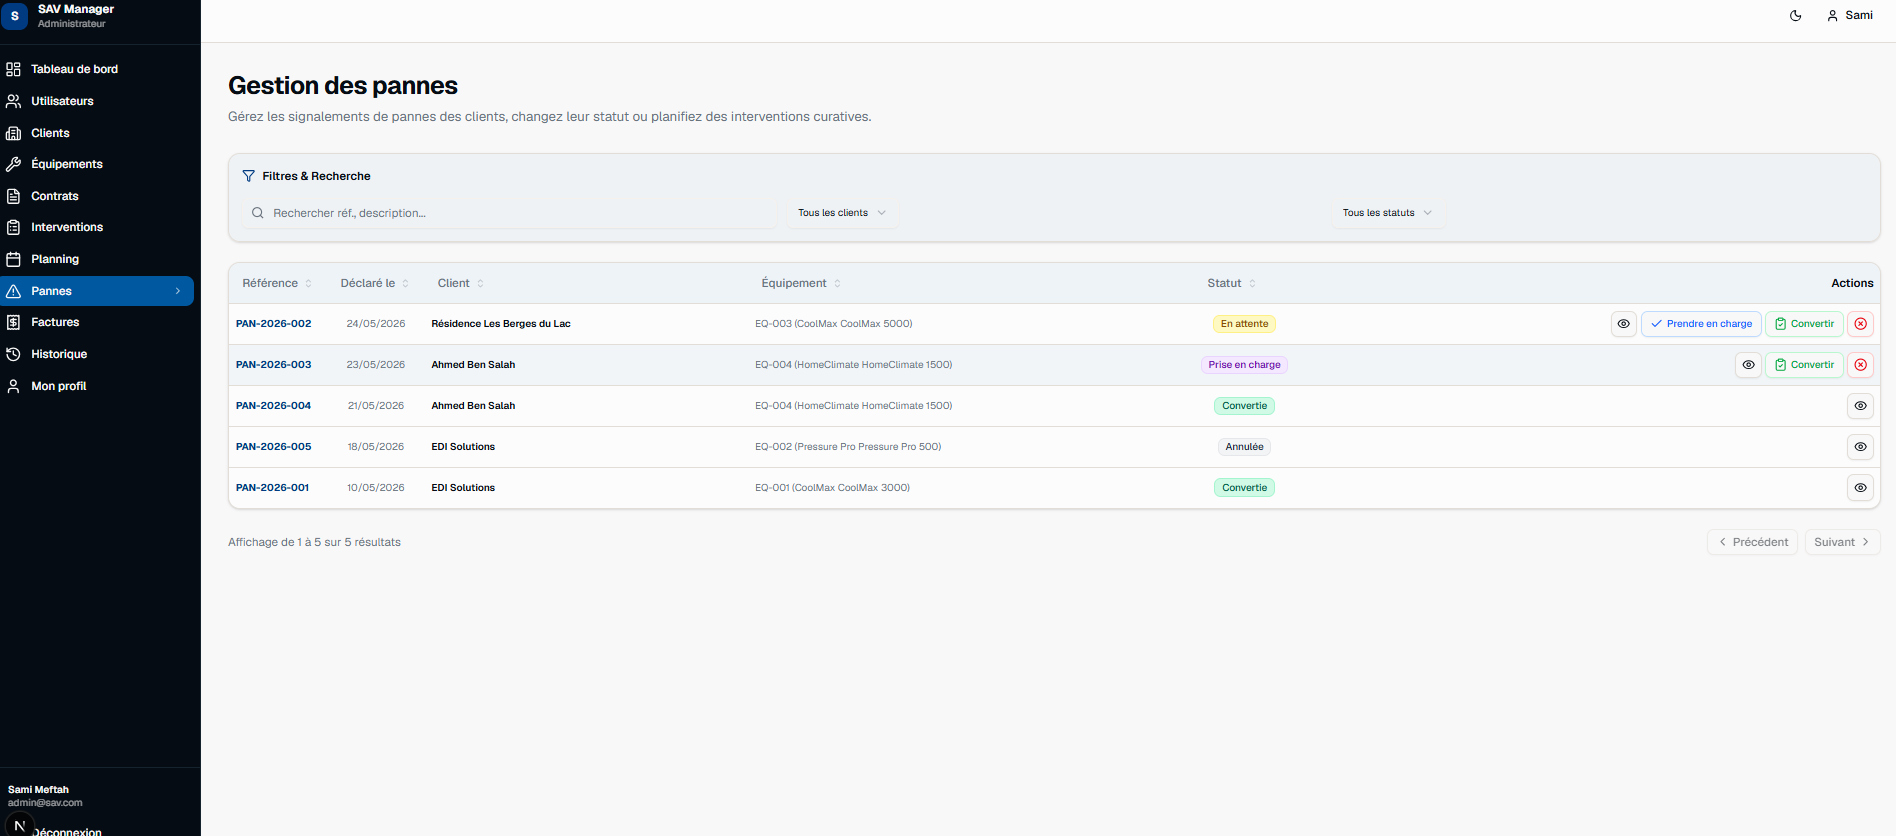
\includegraphics[width=0.74\textwidth]{Figures/Chapitre4/gestpannes.png}
    \caption{Capture d'écran : gestion des pannes}
    \label{fig:ch4:gestion_pannes}
\end{figure}

\begin{figure}[H]
\centering
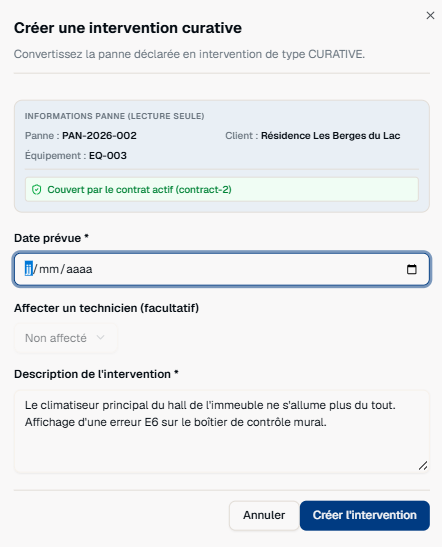
\includegraphics[width=0.45\textwidth]{Figures/Chapitre4/convertirpanne.png}
\caption{Capture d'écran : conversion d'une panne en intervention curative}
\label{fig:ch4:realisation_sprint2_pannes}
\end{figure}

% ─────────────────────────────────────────────────────────────────────────────
\section*{Conclusion}

Ce sprint a permis de développer le cœur fonctionnel du système SAV : la gestion complète du
cycle de vie des interventions préventives et curatives, la déclaration de pannes avec pièces
jointes par les clients, la conversion de pannes en interventions curatives, et la vérification
automatique de la couverture contractuelle. Le chapitre suivant présente le Sprint 3, dédié à la
facturation et aux tableaux de bord.

\newpage
\pagestyle{fancy}
\lhead{\textsc{Chapitre 5. Sprint 3 --- Facturation et tableau de bord}}
\renewcommand{\headrulewidth}{0.5pt}
\renewcommand{\footrulewidth}{0.5pt}
\chapter{Sprint 3 --- Facturation et tableau de bord}\setlength{\headheight}{28pt}
\label{ch5}
\thispagestyle{empty}
\minitoc
\newpage

\section{Introduction}

Suite à l'implémentation des fonctionnalités d'authentification, de gestion du référentiel métier et
de gestion des interventions lors des sprints précédents, ce troisième sprint se concentre sur les
fonctionnalités de supervision et de suivi général du système.

Ce sprint a pour objectif de compléter l'application en y intégrant :

\begin{itemize}
    \item La génération des factures pour les interventions curatives hors contrat ;
    \item Le marquage des factures comme payées ;
    \item L'historique des interventions, différencié par rôle ;
    \item Les tableaux de bord différenciés (administrateur, technicien, client).
\end{itemize}

% ─────────────────────────────────────────────────────────────────────────────
\section{Backlog du Sprint 3}

\begin{longtable}{|p{1.2cm}|p{7.5cm}|p{2.8cm}|p{1.8cm}|}
\caption{Backlog du Sprint 3}
\label{tab:ch5:backlog_sprint3} \\
\hline
\textbf{ID} & \textbf{User Story} & \textbf{Acteur} & \textbf{Priorité} \\
\hline
\endfirsthead
\caption*{Backlog du Sprint 3 (suite)} \\
\hline
\textbf{ID} & \textbf{User Story} & \textbf{Acteur} & \textbf{Priorité} \\
\hline
\endhead
\hline
\endfoot
\hline
\endlastfoot
US-19 & En tant qu'administrateur, je veux générer une facture pour une intervention curative réalisée hors contrat (TVA 19\,\%, TND). & Administrateur & Élevée \\
\hline
US-20 & En tant qu'administrateur, je veux marquer une facture comme payée. & Administrateur & Élevée \\
\hline
US-21 & En tant qu'administrateur, je veux consulter toutes les factures avec filtres (statut, client, date). & Administrateur & Élevée \\
\hline
US-24 & En tant que client, je veux consulter l'historique des interventions sur mes équipements. & Client & Moyenne \\
\hline
US-25 & En tant qu'administrateur, je veux consulter un tableau de bord global avec KPIs et graphiques. & Administrateur & Élevée \\
\hline
US-26 & En tant que technicien, je veux consulter mon tableau de bord personnel. & Technicien & Élevée \\
\hline
US-27 & En tant que client, je veux consulter mon espace personnel. & Client & Élevée \\
\hline
\end{longtable}

% ─────────────────────────────────────────────────────────────────────────────
\section{Analyse}

\subsection{Diagramme de cas d'utilisation du Sprint 3}

\begin{figure}[H]
\centering
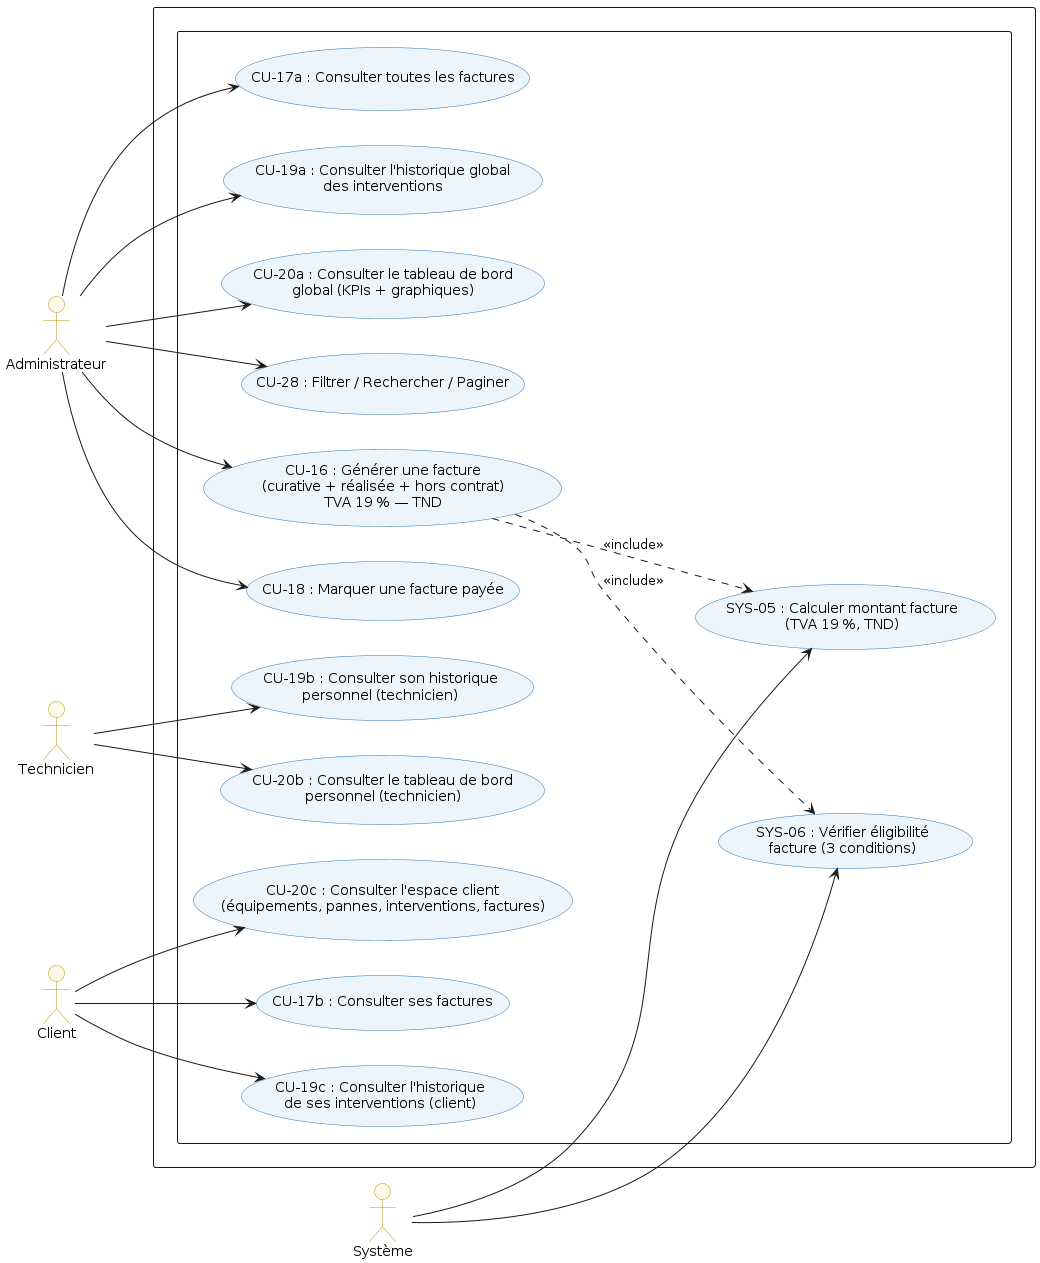
\includegraphics[width=0.70\textwidth]{Figures/Chapitre5/use_case_sprint3.png}
\caption{Diagramme de cas d'utilisation du Sprint 3}
\label{fig:ch5:use_case_sprint3}
\end{figure}

Les acteurs impliqués dans ce sprint sont :

\textbf{Administrateur} : génération et consultation des factures, marquage payée, historique global,
tableau de bord administrateur.

\textbf{Technicien} : consultation de son historique, consultation de son tableau de bord personnel.

\textbf{Client} : consultation de ses factures, de son historique, de son espace personnel.

\subsection{Description des cas d'utilisation}

\subsubsection{CU-16 : Générer une facture}

\begin{table}[H]
\centering
\caption{CU-16 : Générer une facture}
\label{tab:ch5:cu16}
\begin{tabular}{|p{3.5cm}|p{11cm}|}
\hline
\textbf{Champ} & \textbf{Contenu} \\
\hline
Description & Ce cas d'utilisation permet à l'administrateur de générer une facture pour une
intervention éligible. \\
\hline
Acteur principal & Administrateur \\
\hline
Préconditions & L'administrateur est authentifié ; une intervention curative réalisée et hors
couverture contractuelle existe. \\
\hline
Postconditions & La facture est créée et enregistrée dans la base de données. \\
\hline
\end{tabular}
\end{table}

\textbf{Règles d'éligibilité (trois conditions cumulatives) :}

\begin{itemize}
    \item Type de l'intervention = \texttt{CURATIVE}
    \item Statut de l'intervention = \texttt{REALISEE}
    \item Couverture contractuelle = false (\texttt{couvertureContrat} = false)
\end{itemize}

\textbf{Scénario nominal :}

\begin{enumerate}
    \item L'administrateur accède à la liste des interventions éligibles à la facturation.
    \item Il sélectionne une intervention répondant aux trois conditions.
    \item Il saisit les lignes de détail de la facture (\texttt{LigneFacture}) : main-d'œuvre et matériel utilisé.
    \item L'Interface transmet les données au Contrôleur.
    \item Le Contrôleur vérifie les trois conditions d'éligibilité.
    \item Le Contrôleur calcule le montant HT (somme des lignes), la TVA (19\,\%) et le montant TTC.
    \item La base de données enregistre la facture et ses lignes de détail.
    \item La base confirme la création.
    \item L'Interface affiche la facture générée.
\end{enumerate}

\textbf{Règles de gestion :}

\begin{itemize}
    \item \textbf{Les interventions préventives ne génèrent jamais de facture.}
    \item \textbf{Les interventions curatives couvertes par un contrat actif ne génèrent pas de facture.}
    \item La TVA est de \textbf{19\,\%} : \texttt{montantTTC} = \texttt{montantHT} $\times$ 1,19.
    \item La monnaie est le \textbf{Dinar Tunisien (TND)}.
    \item La facture est créée avec le statut \texttt{IMPAYEE} ou \texttt{EN\_ATTENTE}.
\end{itemize}

\textit{Mise à jour du statut de paiement :} Après génération, l'administrateur peut mettre à jour l'état de paiement de la facture (passage au statut \texttt{PAYEE}).

\subsubsection{CU-17 : Consulter les factures}

\begin{table}[H]
\centering
\caption{CU-17 : Consulter les factures}
\label{tab:ch5:cu17}
\begin{tabular}{|p{3.5cm}|p{11cm}|}
\hline
\textbf{Champ} & \textbf{Contenu} \\
\hline
Description & Ce cas d'utilisation permet de consulter les factures selon les droits d'accès. \\
\hline
Acteurs & Administrateur, Client \\
\hline
Préconditions & L'utilisateur est authentifié. \\
\hline
Postconditions & Les factures accessibles à l'utilisateur sont affichées en lecture seule. \\
\hline
\end{tabular}
\end{table}

\textbf{Scénario nominal :} L'utilisateur accède au module des factures ; le système filtre selon le rôle (toutes pour l'administrateur, uniquement les siennes pour le client) et affiche les résultats avec les filtres disponibles.

\textbf{Règles de gestion :}

\begin{itemize}
    \item Le client ne peut consulter que ses propres factures.
    \item La consultation est en lecture seule pour le client.
    \item L'administrateur peut appliquer des filtres par statut, client et date d'émission.
\end{itemize}

\subsubsection{CU-19 : Consulter le tableau de bord administrateur}

\begin{table}[H]
\centering
\caption{CU-19 : Consulter le tableau de bord administrateur}
\label{tab:ch5:cu19}
\begin{tabular}{|p{3.5cm}|p{11cm}|}
\hline
\textbf{Champ} & \textbf{Contenu} \\
\hline
Description & Permet à l'administrateur de consulter les indicateurs globaux du système SAV. \\
\hline
Acteur principal & Administrateur \\
\hline
Préconditions & L'administrateur est authentifié ; des données existent dans le système. \\
\hline
Postconditions & Les statistiques et graphiques sont affichés. \\
\hline
\end{tabular}
\end{table}

\textbf{Contenu du tableau de bord :} KPIs globaux (interventions, contrats, clients, équipements), chiffre d'affaires mensuel, factures impayées, graphiques d'activité mensuelle et répartition préventif/curatif.

\subsubsection{CU-20 : Consulter le tableau de bord technicien}

\begin{table}[H]
\centering
\caption{CU-20 : Consulter le tableau de bord technicien}
\label{tab:ch5:cu20}
\begin{tabular}{|p{3.5cm}|p{11cm}|}
\hline
\textbf{Champ} & \textbf{Contenu} \\
\hline
Description & Permet au technicien de consulter son tableau de bord personnel. \\
\hline
Acteur principal & Technicien \\
\hline
Préconditions & Le technicien est authentifié. \\
\hline
Postconditions & Les indicateurs personnels et le planning du technicien sont affichés. \\
\hline
\end{tabular}
\end{table}

\textbf{Contenu du tableau de bord :} Nombre d'interventions assignées, taux de réalisation, planning de la semaine en cours et dernières interventions réalisées.

\subsubsection{CU-21 : Consulter l'espace client}

\begin{table}[H]
\centering
\caption{CU-21 : Consulter l'espace client (dashboard client)}
\label{tab:ch5:cu21}
\begin{tabular}{|p{3.5cm}|p{11cm}|}
\hline
\textbf{Champ} & \textbf{Contenu} \\
\hline
Description & Permet au client de consulter un résumé de sa situation dans le système. \\
\hline
Acteur principal & Client \\
\hline
Préconditions & Le client est authentifié. \\
\hline
Postconditions & L'espace personnel du client est affiché. \\
\hline
\end{tabular}
\end{table}

\textbf{Contenu de l'espace client :} Équipements affectés, interventions en cours, pannes ouvertes et factures en attente de paiement.

\subsubsection{CU-22 : Consulter l'historique des interventions}

\begin{table}[H]
\centering
\caption{CU-22 : Consulter l'historique des interventions}
\label{tab:ch5:cu22}
\begin{tabular}{|p{3.5cm}|p{11cm}|}
\hline
\textbf{Champ} & \textbf{Contenu} \\
\hline
Description & Permet de consulter l'historique des interventions réalisées ou annulées, filtré selon le rôle. \\
\hline
Acteurs & Administrateur, Technicien, Client \\
\hline
Préconditions & L'utilisateur est authentifié. \\
\hline
Postconditions & L'historique filtré selon le rôle est affiché. \\
\hline
\end{tabular}
\end{table}

\textbf{Scénario nominal :}

\begin{enumerate}
    \item L'utilisateur ouvre le module Historique.
    \item Le Contrôleur filtre les interventions selon le rôle :
    \begin{itemize}
        \item Administrateur $\rightarrow$ toutes les interventions avec statut \texttt{REALISEE} ou \texttt{ANNULEE}.
        \item Technicien $\rightarrow$ uniquement ses interventions assignées avec ces statuts.
        \item Client $\rightarrow$ uniquement les interventions liées à ses \texttt{ClientEquipement}.
    \end{itemize}
    \item Les résultats sont affichés avec filtres (date, type, statut, client, technicien selon le rôle).
\end{enumerate}

Des filtres permettent de faciliter la consultation de l'historique et des tableaux de bord.

% ─────────────────────────────────────────────────────────────────────────────
\section{Conception}

\subsection{Diagramme de classes du Sprint 3}

\begin{figure}[H]
\centering
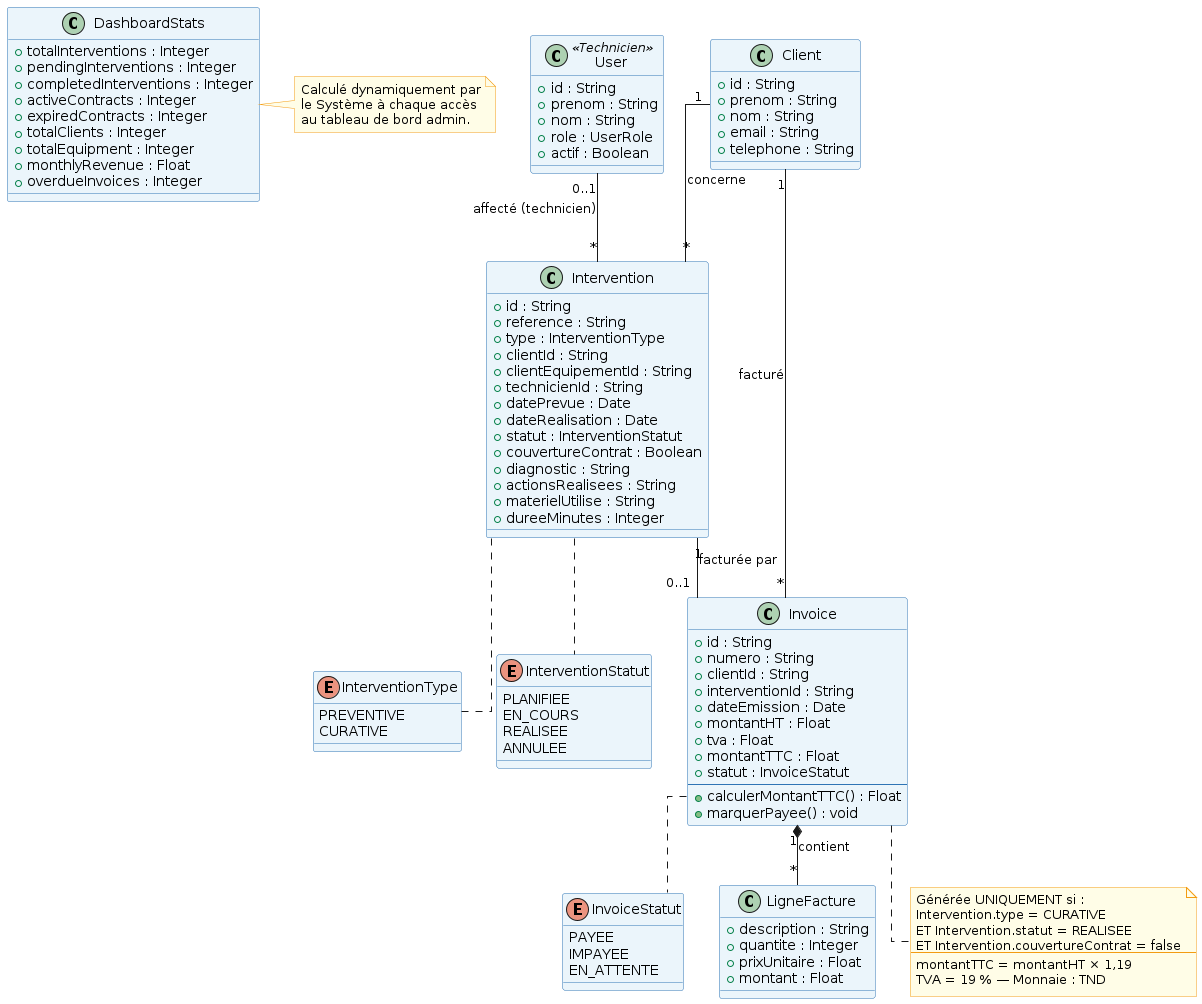
\includegraphics[width=0.70\textwidth]{Figures/Chapitre5/class_diagram_sprint3.png}
\caption{Diagramme de classes du Sprint 3}
\label{fig:ch5:class_sprint3}
\end{figure}

Les entités impliquées dans ce sprint sont : \texttt{Facture}, \texttt{LigneFacture},
\texttt{Intervention}, \texttt{Contract}, Client, User.

\subsection{Diagrammes de séquence}

\subsubsection{Diagramme de séquence : Génération d'une facture}

\begin{figure}[H]
\centering
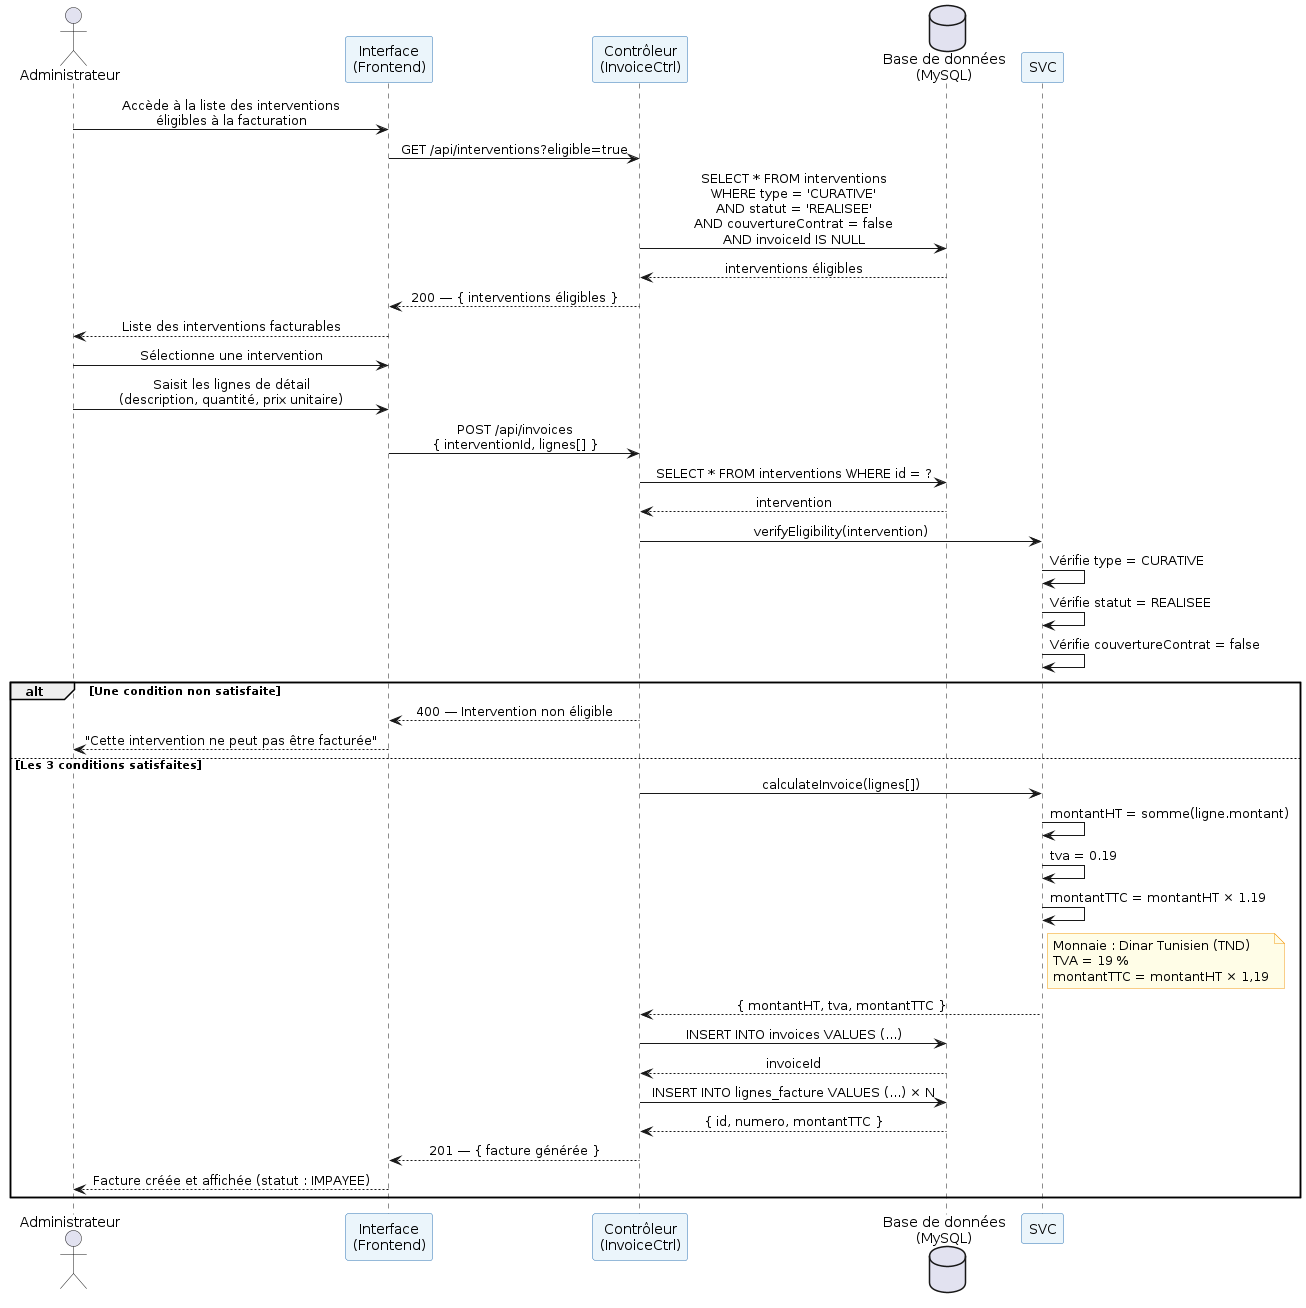
\includegraphics[width=0.70\textwidth]{Figures/Chapitre5/seq_genererfacture_sprint3.png}
\caption{Diagramme de séquence : Génération d'une facture}
\label{fig:ch5:seq_generation_facture}
\end{figure}
\subsubsection{Diagramme de séquence : Consultation de l'historique côté client}

\begin{figure}[H]
\centering
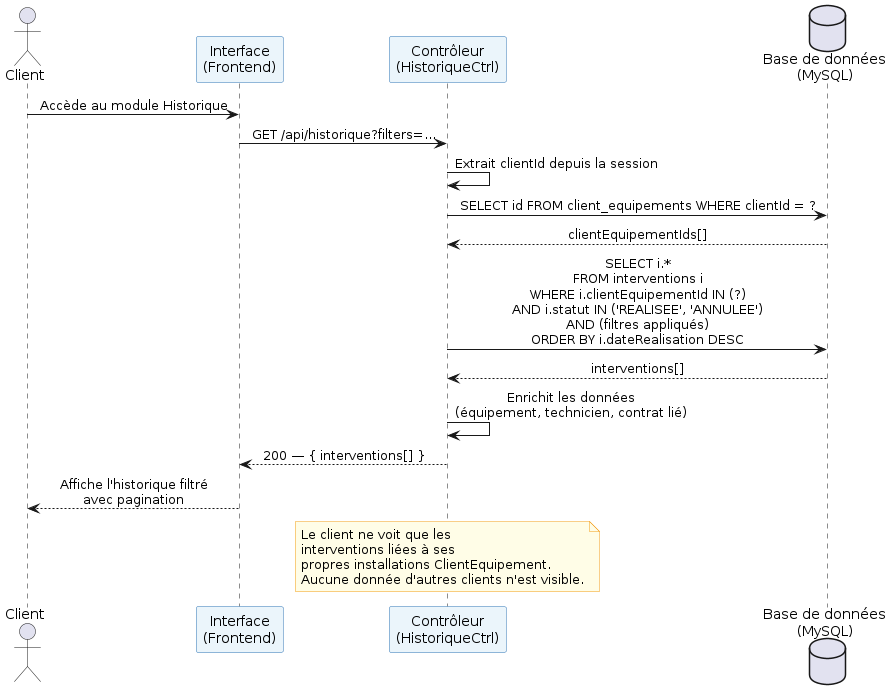
\includegraphics[width=0.70\textwidth]{Figures/Chapitre5/seq_historiqueclient_sprint3.png}
\caption{Diagramme de séquence : Consultation de l'historique côté client}
\label{fig:ch5:seq_historique_client}
\end{figure}

% ─────────────────────────────────────────────────────────────────────────────
\section{Réalisation}

\begin{figure}[H]
\centering
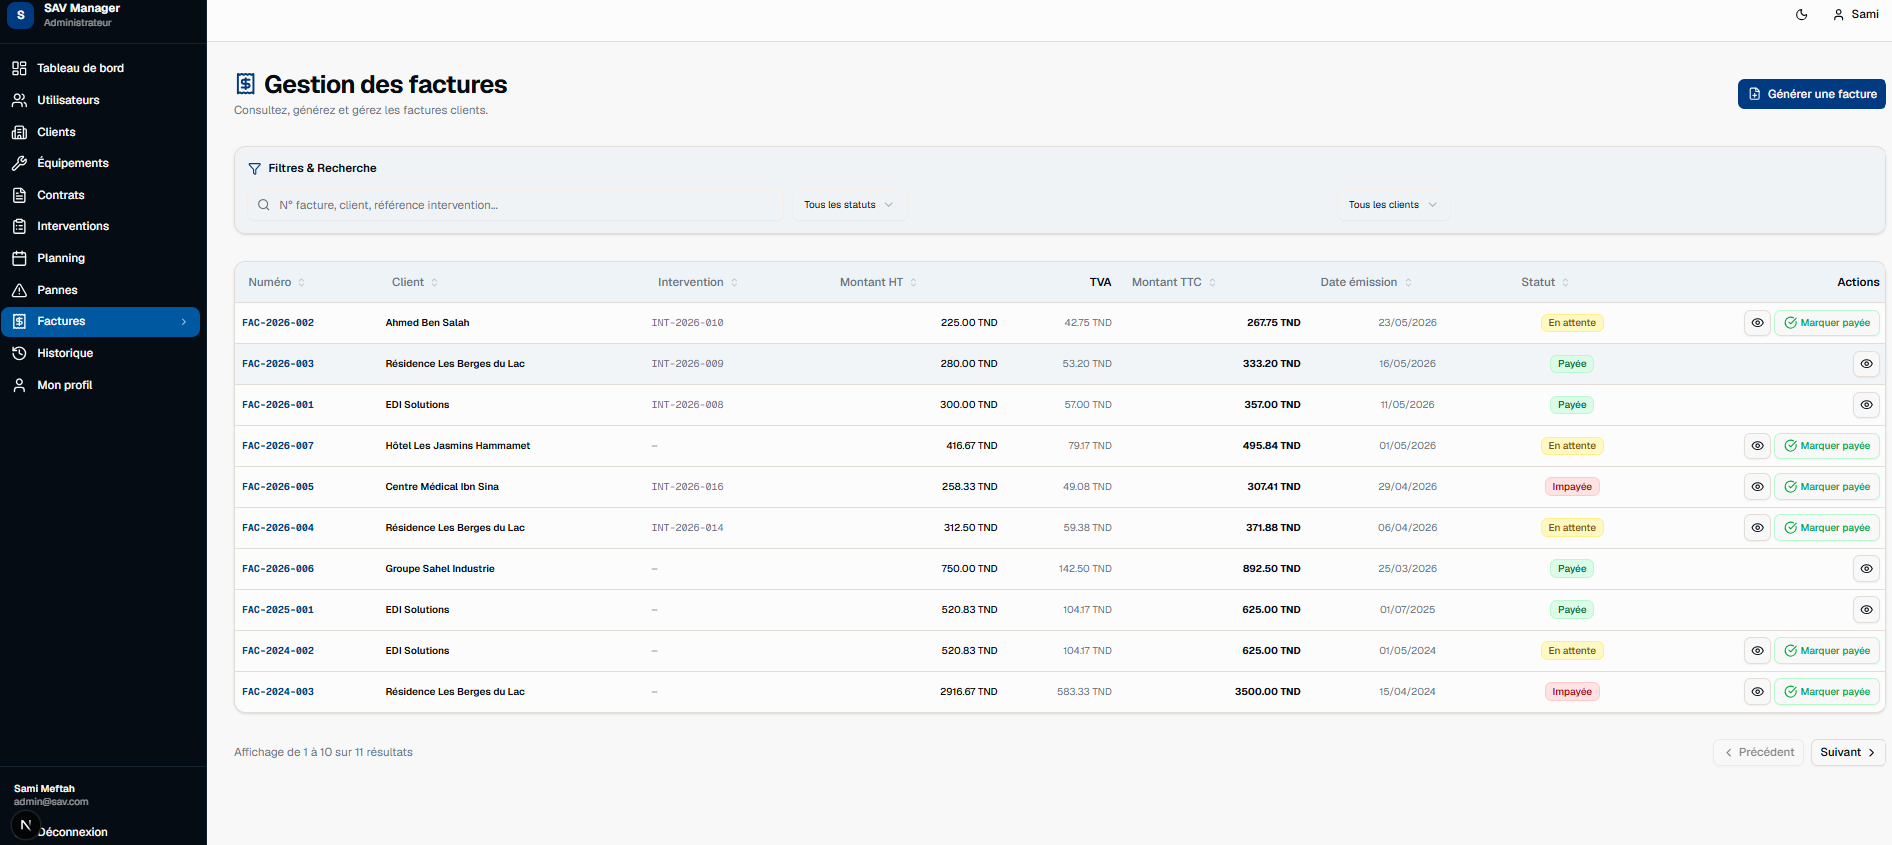
\includegraphics[width=0.65\textwidth]{Figures/Chapitre5/gestfacture.png}
\caption{Capture d'écran de la gestion des factures}
\label{fig:ch4:gestion_factures}
\end{figure}

\begin{figure}[H]
    \centering
    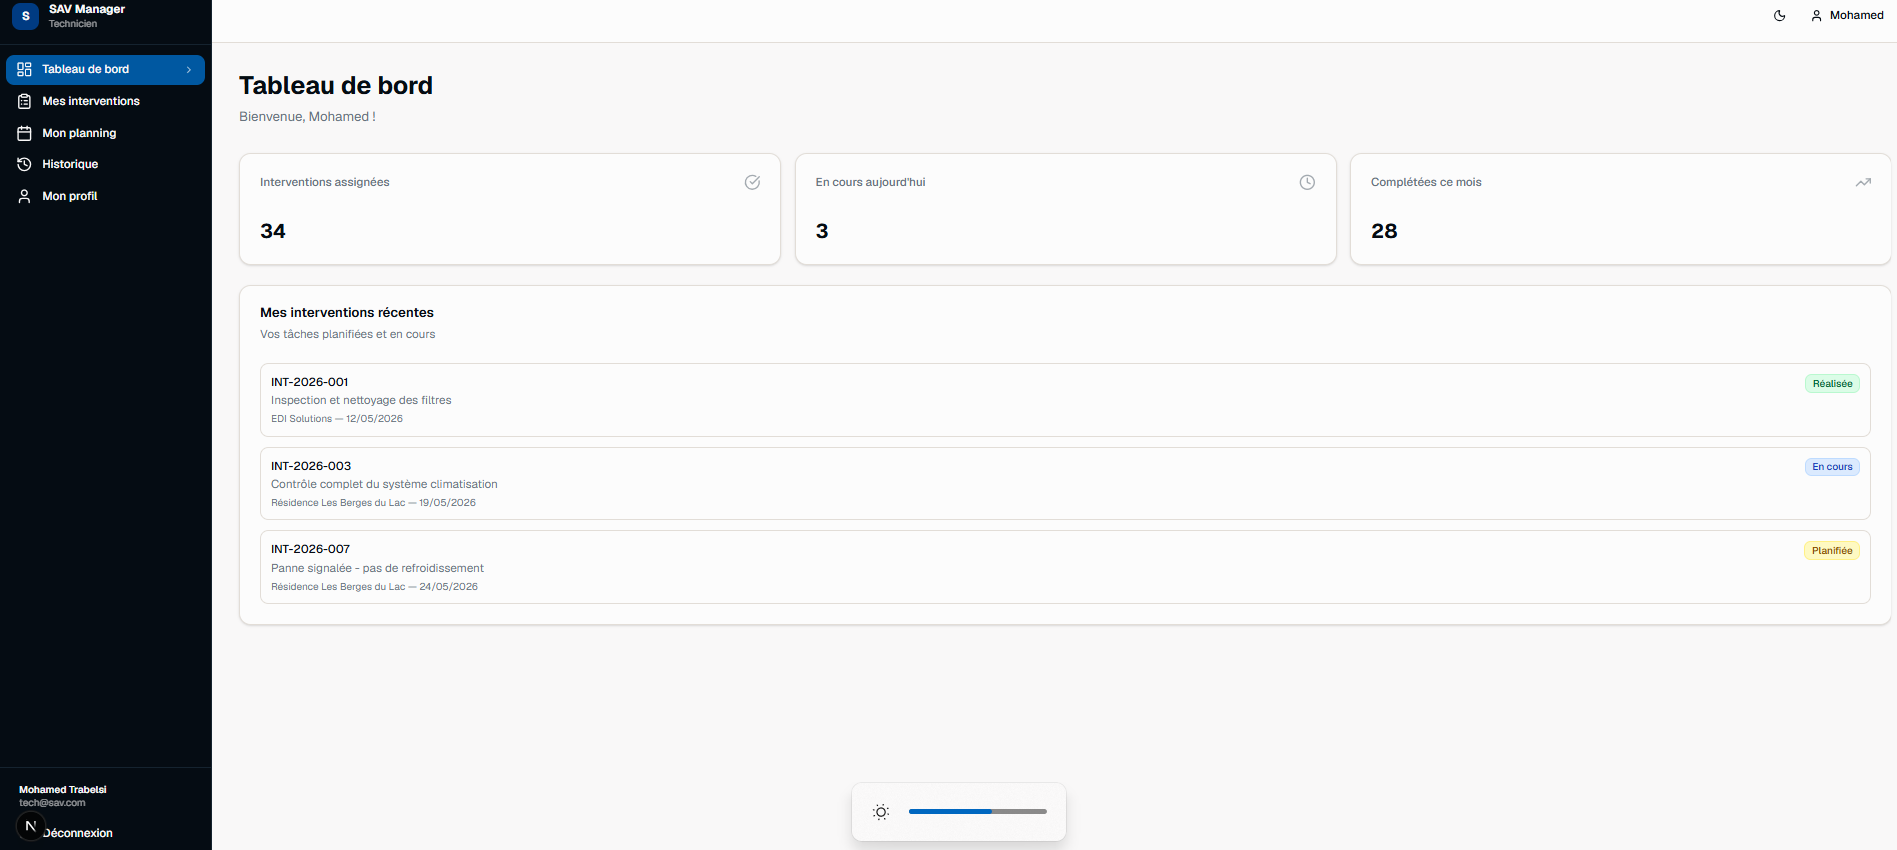
\includegraphics[width=0.74\textwidth]{Figures/Chapitre5/dashboardtech.png}
    \caption{Capture d'écran : tableau de bord technicien}
    \label{fig:ch5:dashboard_technicien}
\end{figure}

\begin{figure}[H]
    \centering
    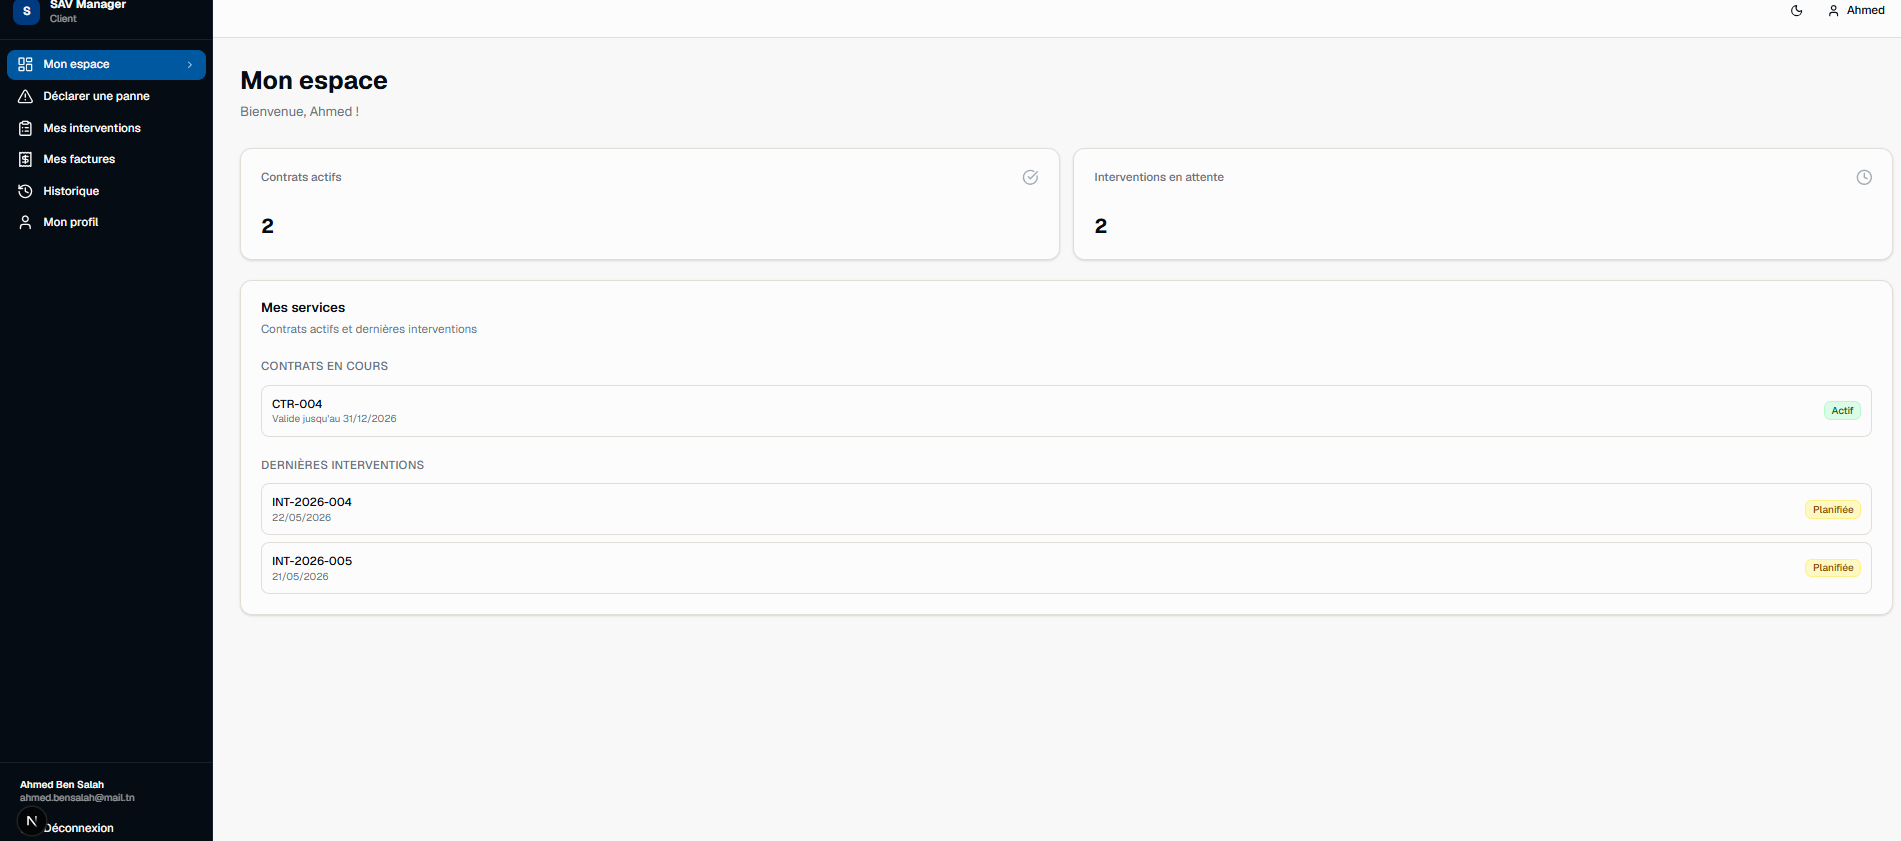
\includegraphics[width=0.74\textwidth]{Figures/Chapitre5/dashboardclientpart.png}
    \caption{Capture d'écran : tableau de bord client}
    \label{fig:ch5:dashboard_client}
\end{figure}

% ─────────────────────────────────────────────────────────────────────────────
\section*{Conclusion}

Ce sprint a permis de finaliser le système SAV avec les fonctionnalités de pilotage : génération
des factures selon les règles d'éligibilité strictes (curative + réalisée + hors contrat), calcul
automatique de la TVA à 19\,\% en dinar tunisien, marquage des factures payées, et des tableaux de
bord différenciés pour l'administrateur, le technicien et le client.


\cleardoublepage
\phantomsection
\addcontentsline{toc}{chapter}{Conclusion Générale}
\newpage
\pagestyle{fancy}
\lhead{\textsc{Conclusion Générale}}
\renewcommand{\headrulewidth}{0.5pt}
\renewcommand{\footrulewidth}{0.5pt}
\chapter*{Conclusion Générale}
\mtcaddchapter

Ce projet de fin d'études a abouti à la conception et au développement d'une application web de
gestion du service après-vente, spécialisée dans la maintenance des climatiseurs et des systèmes
de surpression.

L'application offre une solution complète et intégrée pour digitaliser les processus SAV :

\textbf{Un référentiel métier structuré} : catalogue d'équipements indépendant des clients,
relation \texttt{ClientEquipement} pour matérialiser les installations, gestion des contrats avec
génération automatique du planning préventif.

\textbf{Une gestion opérationnelle complète} : cycle de vie des interventions préventives et
curatives, déclaration de pannes avec pièces jointes, conversion panne $\rightarrow$ intervention,
vérification de disponibilité des techniciens.

\textbf{Un suivi financier automatisé} : facturation conditionnelle (curative + réalisée + hors
contrat), calcul automatique de la TVA à 19\,\%, gestion des statuts de paiement.

\textbf{Des espaces différenciés par rôle} : tableau de bord global pour l'administrateur, tableau
de bord personnel pour le technicien, espace client dédié.

Sur le plan technique, ce projet a permis de maîtriser une architecture moderne en trois couches
(Frontend Next.js/React, Backend API, Base de données Prisma/MySQL) avec Prisma ORM garantissant
la séparation des préoccupations et l'intégrité transactionnelle des données.

La méthodologie Scrum adoptée a permis un développement itératif et incrémental, avec trois sprints
progressifs couvrant l'ensemble du périmètre fonctionnel.

Ce projet constitue une base solide pour une mise en production future, avec des perspectives
d'évolution comme l'intégration de notifications temps réel, la génération de rapports d'activité
avancés ou l'extension à d'autres types d'équipements de maintenance.


% ===== Perspectives =====
\cleardoublepage
\phantomsection
\addcontentsline{toc}{chapter}{Perspectives}
\chapter*{Perspectives}
\thispagestyle{empty}
Ce projet ouvre la voie à plusieurs perspectives d'amélioration et d'extension :

\begin{itemize}
    \item Intégration d'un système de notifications en temps réel afin d'alerter les techniciens et les administrateurs lors de nouvelles interventions ou pannes déclarées.
    \item Développement d'une application mobile dédiée permettant aux techniciens d'accéder aux informations terrain directement depuis leurs appareils.
    \item Génération de rapports d'activité avancés et personnalisables pour un meilleur suivi des performances du service après-vente.
    \item Optimisation automatique de la planification des interventions préventives grâce à des algorithmes intelligents tenant compte de la disponibilité des techniciens et de la charge de travail.
    \item Extension du système à d'autres types d'équipements techniques, au-delà des climatiseurs et des systèmes de surpression.
\end{itemize}


% ===== Webographie =====
\clearpage
\pagestyle{empty}
\phantomsection
\addcontentsline{toc}{chapter}{Webographie}
\chapter*{Webographie}
\thispagestyle{empty}
\markboth{Webographie}{Webographie}

% ===== Résumé (Quatrième de couverture) =====
\cleardoublepage
\pagestyle{empty}
\thispagestyle{empty}
\section*{Résumé}
\addcontentsline{toc}{chapter}{Résumé}

\textit{[À compléter]}

\bigskip

\section*{Mots-clés}

\textit{[À compléter]}

\bigskip
\newpage

\section*{Abstract}
\addcontentsline{toc}{chapter}{Abstract}

\textit{[To be completed]}

\bigskip

\section*{Keywords}

\textit{[To be completed]}

\end{document}
